\RequirePackage[l2tabu,orthodox]{nag}

% TODO: decide if one-sided/two-sided
%\documentclass[headsepline,footsepline,footinclude=false,fontsize=11pt,paper=a4,listof=totoc,bibliography=totoc,BCOR=12mm,DIV=12]{scrbook} % two-sided
\documentclass[headsepline,footsepline,footinclude=false,oneside,fontsize=11pt,paper=a4,listof=totoc,bibliography=totoc]{scrbook} % one-sided

\PassOptionsToPackage{table,svgnames,dvipsnames}{xcolor}

\usepackage[utf8]{inputenc}
\usepackage[T1]{fontenc}
\usepackage[sc]{mathpazo}
\usepackage[american]{babel}
\usepackage[autostyle]{csquotes}
\usepackage[%
  backend=biber,
  url=false,
  style=alphabetic,
  maxnames=4,
  minnames=3,
  maxbibnames=99,
  firstinits,
  uniquename=init]{biblatex} % TODO: adapt bibliography style
\usepackage{graphicx}
\usepackage{scrhack} % necessary for listings package
\usepackage{listings}
\usepackage{lstautogobble}
\usepackage{tikz}
\usepackage{multirow}
\usepackage{amsmath}
\usepackage{amssymb}
\usepackage{url}
\usepackage{csquotes}
\usepackage{pgfplots}
\usepackage{pgfplotstable}
\usepackage{booktabs}
\usepackage[final]{microtype}
\usepackage{caption}
\usepackage[hidelinks]{hyperref} % hidelinks removes colored boxes around references and links
\usepackage[toc,nonumberlist,acronym]{glossaries} % TODO: remove if glossary not needed

\bibliography{bibliography/literature}

\setkomafont{disposition}{\normalfont\bfseries} % use serif font for headings
\linespread{1.05} % adjust line spread for mathpazo font

% Settings for glossaries TODO: remove the following block if glossary not needed
\renewcommand{\glsnamefont}[1]{\normalfont\bfseries #1} % use serif font for glossary entry titles
\makeglossaries{}

% Settings for pgfplots
\pgfplotsset{compat=1.9} % TODO: adjust to your installed version
\pgfplotsset{
  % For available color names, see http://www.latextemplates.com/svgnames-colors
  cycle list={CornflowerBlue\\Dandelion\\ForestGreen\\BrickRed\\},
}

% Settings for lstlistings
\lstset{%
  basicstyle=\ttfamily,
  columns=fullflexible,
  autogobble,
  keywordstyle=\bfseries\color{MediumBlue},
  stringstyle=\color{DarkGreen}
}

% Basic information for cover & title page
\newcommand*{\getUniversity}{Technische Universität München}
\newcommand*{\getFaculty}{Fakultät für Informatik}
\newcommand*{\getTitle}{Efficient Data Mining Algorithms in Main Memory Databases}
\newcommand*{\getTitleGer}{Effiziente Data Mining Algorithmen in Hauptspeicher-Datenbanken}
\newcommand*{\getAuthor}{Martin Kapfhammer}
\newcommand*{\getDoctype}{Master's Thesis in Informatics}
\newcommand*{\getSupervisor}{Linnea Passing, M.Sc.}
\newcommand*{\getAdvisor}{Prof. Alfons Kemper, Ph.D.}
\newcommand*{\getSubmissionDate}{15.04.2015}
\newcommand*{\getSubmissionLocation}{Munich}

% TODO: add custom commands etc.


% TODO: remove if glossary not needed
\newglossaryentry{computer}
{
  name=computer,
  description={is a machine that\ldots}
}

\newacronym{tum}{TUM}{Technische Universität München}


\begin{document}

\begin{titlepage}
  % HACK for two-sided documents: ignore binding correction for cover page.
  % Adapted from Markus Kohm's KOMA-Script titlepage=firstiscover handling.
  % See http://mirrors.ctan.org/macros/latex/contrib/koma-script/scrkernel-title.dtx,
  % \maketitle macro.
  \oddsidemargin=\evensidemargin\relax
  \textwidth=\dimexpr\paperwidth-2\evensidemargin-2in\relax
  \hsize=\textwidth\relax

  \centering

  \vspace{40mm}
  
\includegraphics[width=40mm]{logos/tum}

  \vspace{5mm}
  {\huge\MakeUppercase{\getFaculty{}}}\\

  \vspace{5mm}
  {\large\MakeUppercase{\getUniversity{}}}\\

  \vspace{20mm}
  {\Large \getDoctype{}}

  \vspace{15mm}
  {\huge\bfseries \getTitle{}}

  \vspace{15mm}
  {\LARGE \getAuthor{}}

  \vspace{20mm}
  
\includegraphics[width=20mm]{logos/faculty}
\end{titlepage}


\frontmatter{}

\begin{titlepage}
  \centering

  \vspace{40mm}
  
\includegraphics[width=40mm]{logos/tum}

  \vspace{5mm}
  {\huge\MakeUppercase{\getFaculty{}}}\\

  \vspace{5mm}
  {\large\MakeUppercase{\getUniversity{}}}\\

  \vspace{20mm}
  {\Large \getDoctype{}}

  \vspace{15mm}
  {\huge\bfseries \getTitle{}}

  \vspace{10mm}
  {\huge\bfseries \getTitleGer{}}

  \vspace{15mm}
  \begin{tabular}{l l}
    Author: & \getAuthor{} \\
    Supervisor: & \getSupervisor{} \\
    Advisor: & \getAdvisor{} \\
    Submission Date: & \getSubmissionDate{} \\
  \end{tabular}

  \vspace{20mm}
  
\includegraphics[width=20mm]{logos/faculty}
\end{titlepage}

\thispagestyle{empty}
\vspace*{0.8\textheight}
\noindent
I assure the single handed composition of this \MakeLowercase{\getDoctype{}} only supported by declared resources.

\vspace{15mm}
\noindent
\getSubmissionLocation{}, \getSubmissionDate{} \hspace{5cm} \getAuthor{}

\cleardoublepage{}

\addcontentsline{toc}{chapter}{Acknowledgments}
\thispagestyle{empty}

\vspace*{2cm}

\begin{center}
{\usekomafont{section} Acknowledgments}
\end{center}

\vspace{1cm}

I would like to thank my supervisors, Prof. Alfons Kemper, Ph.D. and Prof. Dr. Thomas Neumann and my advisor, Linnea Passing, M.Sc., for the opportunity to work on this thesis, their useful comments, remarks and engagement throughout the work.

\cleardoublepage{}

\chapter{\abstractname}

%TODO: Abstract



\microtypesetup{protrusion=false}
\tableofcontents{}
\microtypesetup{protrusion=true}

\mainmatter{}

\chapter{Introduction}\label{chapter:introduction}

\section{Motivation}


Databases are more in the center of innovation than ever. With the growing demands on storing and analyzing large amounts of data, linked with the capabilities of modern hardware, database vendors and researchers face new challenges and possibilities. 
\\
Traditionally, databases are disk-based systems separated into two parts: One system used for Online Transactional Processing (OLTP), optimized for high rates of mission-critical, transactional write requests. As second system, a data warehouse is used for Online Analytical Processing (OLAP), executing long-running queries to gain insight into the  collected data, used to make future business decisions upon. Due to this contradicting requirements of critical, short write requests on the one side and long running, business-intelligence gaining read requests on the other side, traditionally two separated systems are used. The data synchronization between the two systems is ensured by an ETL process: Data is extracted from the OLTP system, transformed and loaded into the OLAP system. Since this process implicates heavy load on the database, it is usually done periodically, e.g. over night. Obviously, this architecture reveals several drawbacks, like stale data, redundancy and the maintenance cost of two systems.
\\
Modern hardware allows us to move away from this paradigm: Instead of using disk-based databases the data can be stored in memory. Since memory can be accessed much faster than the disk, an unprecedented throughput of OLTP transactions is possible. Using snapshots of the transactional data by exploiting the virtual memory management of the operating system, OLAP queries can run in parallel next to the OLTP transactions on up-to-date data. Such a system is HyPer, a relational main memory database guaranteeing the ACID properties, actively developed at the Chair of Database Systems at the TU München, and the main system used for our research. 
\\
The possibility of executing OLAP queries on a relational DBMS without interfering the OLTP transaction throughput opens new possibilities for database systems. Additionally to long-running OLAP queries, data mining algorithms can be implemented and executed in HyPer. Data mining extends the possibilities of OLAP by applying more compelex algorithms to discover interesting patterns and knowledge from the data. Crucial techniques are mining frequent patterns and association rules, classification, clustering and outlier detection.
\\
Usually data mining tools have to import and integrate data from databases and other data sources by ETL processes, resulting in the same disadvantages as for data warehouses: data is not up-to-date for the crucial analyzing phase and redundant. 
\\
By implementing data mining algorithms right into the database, data analysts, data scientists and business executives gain huge benefits. Instead of bringing the data to the algorithm, the algorithms are brought to the data. No ETL processes are necessary to export data to an additional system for data mining. Instead, the algorithms can be executed directly on the database system on up-to-date data. The execution of the algorithms can benefit from the modern hardware and high computational power of the database system. Additionaly, the data mining process can be combined with already existing database operators such as grouping and aggregation, resulting in a very natural environment for data analysis.


\section{Research Questions}
With more and more data generated by modern IT systems, the needs for analyzing large amounts of data are rapidly growing and data mining software gets an increasing amount of attention. So far, most data scientists use standalone data mining tools such as R~\parencite{R/stats}, Julia~\parencite{DBLP:journals/corr/abs-1209-5145} or the Python ecosystem SciPy~\parencite{scipy}. Also the Java frameworks Weka~\parencite{Hall:2009:WDM:1656274.1656278} and ELKI~\parencite{DBLP:conf/ssdbm/AchtertKZ08} are used actively, in particular in the research community. All tools are providing an environement for statistical computing and the application of various data mining algorithms. Additionaly, for mining tera- and petabytes of data, scalable software such as Apache Hadoop~\parencite{hadoop}, Apache Spark~\parencite{spark} and the data mining and machine learning framework Apache Mahout~\parencite{mahout} are used.
\\
While all of the presented environments are frequently used by data scientists, they demonstrate one decisive drawback: Before executing data mining algorithms on the data sets, the data first has to be fetched from the database and transformed into a format readable by these tools. Therefore a first enhancement is to bring the algorithms closer to the database. Tools like MADlib~\parencite{MADlib} and RapidMiner~\parencite{RapidMiner} are supporting specific database engines and trying to fill this gap. Algorithms can be run on the database, using extensible SQL, already existing SQL operators, stored procedures and the possibility to run high-level \enquote{glue} code on the database. These tools provide a middleware between the database and data mining software and therefore data export becomes obsolete. 
\\
However, for complex algorithms SQL operators have to be combined with high-level constructs, often resulting in bad performance. Therefore, database vendors such as Oracle and SAP are providing their databases with more and more statistical and data mining functionalities using existing SQL syntax~\parencite{oracle}~\parencite{SAP}. This leads to several advantages: A database system provides already efficient data storage and access, therefore data mining algorithms implemented on the database can benefit from these data structures. Besides, databases are optimized for modern hardware, e.g. multicore processors and cache hierarchies, which makes them presumably faster than platform-independent tools. Furthermore, data mining algorithms can profit from database features such as parallelization, scalability, recovery and backup facilities as well as from the query language SQL. SQL itself comes already with useful algorithms for data analysis such as selection, sorting and aggregation. Therefore an extension of the query language to integrate other algorithms for data mining would feel very natural to the data scientist. 
\\
Regarding those advantages our research goal is to extend HyPer by data mining functionalities that can be executed directly on the database, exploiting the performance of modern database hardware for computational operations and building a general-purpose system for OLTP, OLAP and data mining queries. 


\section{Approach}
As proof of concept, the well-known k-Means algorithm will be implemented as a HyPer operator. K-Means is one of the most popular  clustering algorithms and available on all presented platforms. Since the algorithm is relatively simple and straightforward, a good comparability between different tools and their performance is given. Since most data mining algorithms are non-deterministic, the time per iteration will be the main criterion. Therefore, the implementation of k-Means should demonstrate the possibilities of implementing and running data mining algorithms in HyPer.
\\
HyPer provides a programming model for the implementation of operators by combining pre-compiled C++ code with dynamically generated LLVM code. Yet, the programmer has a lot of freedom in implementing complex data mining operators. This work compares different implementation aspects of the k-Means algorithm and aims to detect best practices, patterns and building blocks for the implementation of further algorithms.
\\
The remainder of this thesis is organized as follows: In the next section, fundamentals of the HyPer database are presented. In chapter~\ref{chapter:kdd}, a bried introduction of the terms knowledge discovery and data mining is given. Then, the k-Means clustering algorithm is introduced. Chapter~\ref{chapter:related} dicusses other data mining tools and databases with data mining functionalities. In chapter~\ref{chapter:implementation} the implementation of the k-Means clustering algorithm as HyPer operator is depicted. Chapter~\ref{chapter:evaluation} discusses extensive experiments that demonstrate the applicability of data mining algorithms in HyPer. Chapter~\ref{chapter:conclusion} concludes the thesis.




\chapter{HyPer}\label{chapter:hyper}
\section{Motivation}
In this chapter, the relational main memory database system HyPer is introduced. HyPer is a database system combining both OLTP and OLAP processing and is the main research subject of this work: Extending HyPer in order to execute data mining algorithms directly in the relational database.
\\
As already mentioned, historically databases are disk-based systems separated into two parts: An OLTP system, optimized for high rates of mission-critical, transactional write requests, and an OLAP system, executing long-running queries. The data synchronization is ensured by an ETL process that extracts, transforms and loads data from the OLTP to the OLAP system. Since this process implicates heavy load on the database, it is usually done periodically, e.g. over night. 
\\
Obviously, this architecture reveals several drawbacks. The periodical execution of the ETL process results in stale data on the OLAP system, i.e. when implementing a nightly ETL process, data can be outdated for up to 24 hours which can be problematic for real-time data analysis. Furthermore, two systems lead to a higher amount of cost. Hardware and software costs must be taken into account as well as maintenance cost and incident management. Additionally, implementing an ETL process can make a system overly complex in contrast of having one system.
\\
Addressing these challenges the HyPer main memory system was developed, with the goals to process OLTP transactions with high performance and throughput, and, on the same system, process OLAP queries on up-to-date data. 

\section{Architecture}
In this section we give an overview about the HyPer system architecture and important design decisions. Major performance gains of HyPer are realized by omitting typical disk-based database characteristics that are not necessary any more when data resides in main memory. For example, database-specific buffer management and page structuring is not needed. Instead, data is stored in main memory optimized data structures within the virtual memory. Hence, HyPer can use the highly efficient address-translation of the operating system without any additional indirection.
\\
On such a system, OLTP processing is very fast because all the data is already loaded into main memory and slow disk access is omitted and not a bottleneck anymore. Therefore, transactions do never have to wait for I/O and can be executed very quickly. Thus, HyPer implements OLTP transactions as a single-threaded approach and executes all transactions sequentially. This is possible because the execution time of an OLTP transaction is in microseconds and even without parallel execution of transactions, a high throughput is achievable. Another advantage of this simple model is that locking and latching of data objects become redundant since only one transaction is active for the entire database. Even though there are developments to relax these constraints the basic OLTP processing is sequentially.
\\
Obviously, the sequential execution of transactions is only possible if there aren’t any long-running transactions. Long-running transactions would be a bottleneck for the entire database and must be handled in a different way. Therefore we will now look at how HyPer deals with OLAP queries.
\\
HyPer considers OLAP queries as a new process and creates a snapshot of the virtual memory of the OLTP process for its OLAP processes. In Unix, this is done by forking the OLTP process and creating a child process for the OLAP process, exploiting the virtual memory functionality of the operating system. The OLAP process takes an exact copy of the OLTP system on process creation and is now able to execute long running queries without interfering the OLTP transaction throughput. Thanks to modern operating systems the creation of snapshots is very efficient because the memory segments are not physically copied. Instead, operating systems apply a \texttt{copy-on-update strategy}. That means that both OLTP and OLAP processes are sharing the same physical main memory location since their virtual address translation maps to the same segments. Therefore copying memory on creation is not necessary. Only when an object is updated by the OLTP process, a new page gets created for the OLTP process, while the OLAP virtual memory page is still the one available when the process was created. Since this mechanism is supported by hardware, it is very fast and efficient without any implementation overhead for the HyPer database system. Experiments have also shown that a \texttt{fork} can be achieved in several milliseconds, almost independent of the size of the OLTP system.
\\
Since OLAP queries are read-only HyPer can execute them in parallel in multiple threads sharing the same snapshot. As in the sequential execution, locking and latching is not necessary because the used data structures are immutable. This inter-query parallelization can tremendously speed up query processing on multicore computers. Another approach is the creation of multiple OLAP session by forking the OLTP memory periodically. Therefore, for each OLAP session a new virtual memory snapshot is created and used as the current snapshot for the new session. This allows parallelization not only as inter-query parallelization but also among the different OLAP sessions.
\\ 
In this chapter we have shown the advantages of a modern main memory system such as HyPer. Without the bottleneck of disk I/O, database operations can be run sequentially with a high throughput. OLAP queries can run very efficiently in parallel to the OLTP transaction system on different virtual memory snapshots. Due to these possibilties we explore now how to not only execute OLAP queries on a running transactional database but also more complex data mining algorithms.



\chapter{Knowledge Discovery and Data Mining}\label{chapter:kdd}
In this chapter we clarify the terms and importance of knowledge discovery and data mining. Shortly it is the process of gaining knowledge and insight from data.
\section{Motivation}
As already mentioned, data growth is exploding and new data is generated every day by every aspect of daily life, such as businesses, society, science and medicine. With this huge amount of data available, it has become one of the most valuable resources of our decade. Quotes that compare data with the importance of oil or see it as a new currency become more frequent.
\\
However, before data has any value it has to be transformed into knowledge. For example, e-commerce companies are very keen to find out not only what their customers bought but also what they are likely to buy in the future to generate more revenue. Therefore, they are using data mining techniques to present products to their customers in which they might be interested. This products can be similar to products the customer has already bought in the past, or it is a product another customer with similar characteristics has bought in the past. A very well known example is amazon.com which is offering a variety of similar products the customer recently looked for. In that case, data mining is used to boost consumerism. Additionally, this knowledge might be used to optimize storage cost, e.g. by knowing how much of certain products will be needed to distribute in the next weeks.
\\
Other areas for data mining are telecommunication network carriers with a huge amount of data traffic generated every day, the health and medical industry and the Web in general, to name just a few examples. Again it is all about knowledge. The telecommunication network carriers are interested in their customers usage behaviour, while state authorities are interested in wiretapping of potential criminals. Medical data might be used to install an ameliorated patient monitoring and Web data can be used for a search engine to find the best results or deliver promising ads. The list of sources to generate data from and the knowledge one is interested in is endless.


\section{Knowledge Discovery}

After understanding the importance of data mining for gaining knowledge and using this knowledge for further decision making this section defines the data mining steps in greater detail. The term data mining itself often leads to confusion - we are not mining data but instead we are looking for knowledge and interesting patterns in a given data set or database. Therefore, the term knowledge discovery is often more appropriate.


\begin{figure}[htsb]
  \centering
  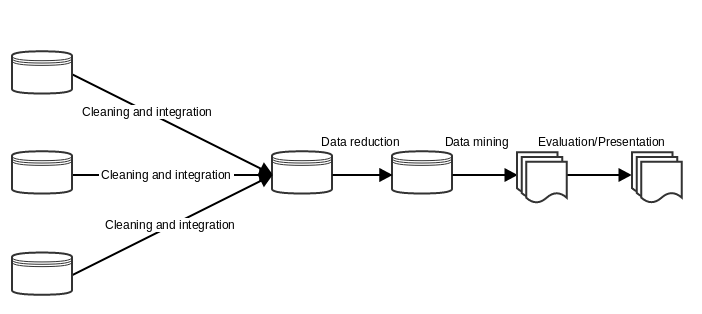
\includegraphics[scale=0.5]{figures/kdd}
  \caption[The Process of Knowledge Discovery]{The Process of Knowledge Discovery.}\label{fig:kdd}
\end{figure}

Usually, data mining is seen as a part of the knowledge discovery process as depicted in~\autoref{fig:kdd}. The knowledge discovery process starts with the preprocessing steps data cleaning, integration, selection and transformation. The actual knowledge gain is then acquired in the data mining step, afterwards the knowledge is evaluated and presented. In this work we use the term data mining as described in ~\autoref{fig:kdd} since we are mainly interested in the algorithms applied in the data mining phase. Nevertheless, in this chapter we give a profound overview over all the knowledge discovery steps.
\\
Regarding all those steps, Han et al.~\parencite{dmbook} give a detailed definition of data mining: 
\begin{quote}
“Data mining is the process of discovering interesting patterns and knowledge from large amounts of data. The data sources can include databases, data warehouses, the Web, other information repositories, or data that are streamed into the system dynamically.”
\end{quote}

In the following sections we look at each phase in detail and start with data cleaning. 

\subsection{Data Cleaning} 
The first step of knowledge discovery needs to ensure that the data we are interested in is complete, clean and consistent. Real world data is usually none of it. Data sets are incomplete, i.e. values are missing. If these missing values are crucial for the further data mining process, several data cleaning techniques exist to fill the gaps in the data, e.g. by using an average value such as the mean or median.
\\
The same is true for inconsistent or redundant data. An example of inconsistent data are distinct values with the same meaning. Additionally, we often see random error or variance in a measured variable. This is called noisy data and must be cleaned for proper data analysis e.g. by smoothing the data set, using binning techniques.


\subsection{Data Integration}

Data mining often requires data from several sources. These sources can be databases, data warehouses, transactional data or plain data files. Also complex data might be used, such as time-related data, data streams, spatial data, multimedia data and graph data. All these sources have to be integrated into one coherent data set which can be used for further analysis. There are several challenges regarding data integration, the most important is the entity identification problem: When combining data from different sources same data objects can have different names and types in different schemas. Therefore, data integration often requires domain knowledge of the different data sources and techniques used in data cleaning to get a clean, consistent data set and to avoid redundancy.


\subsection{Data Reduction}

After cleaning and integrating data into a coherent data set, the data should be ready for further mining. However, those data sets are often of huge size and contain much information, not all necessary for the data mining process. Data reduction techniques can help to reduce the information density and speed up the data analysis and mining process. Simple techniques for data reduction are projection, selection and aggregation, available in every database system. More advanced techniques are dimensionality reduction, e.g. by a principal component analysis, numerosity reduction above aggregation, e.g. clustering or sampling, and data compression. 
\\
Other methods are data transformation which changes the data by converting values into another format e.g. by using normalization. Another possibility is data discretization, e.g. by transforming numeric data into intervals. 
\\
The aim of all of the addressed methods is to reduce the size of the initial data set and therefore to make it easier to get the information the user is interested in. Some methods of the presented data reduction techniques are data mining techniques as well, e.g. clustering. Therefore the boundary between data reduction and data mining is not always easy to draw.


\subsection{Data Mining}

After applying the presented preprocessing steps the data set is now ready for data mining techniques. In the data mining phase we apply algorithms for finding interesting patterns in the data set. Crucial techniques are mining frequent patterns and association rules, classification, clustering and outlier detection. These algorithms are part of section ~\ref{section:datamining}. 


\subsection{Pattern Evaluation}

After generating those patterns we have to evaluate them to figure out how valuable the acquired knowledge is. There exist several criteria for pattern evaluation. First, a pattern has to be understandable. A clustering for example does not give any knowledge if the reason for the clustering is not comprehensible. Therefore, the reasons of a data mining pattern must be clear for the user. That leads to the next criteria of evaluation: A pattern has to be valid, useful and novel. Only then, a pattern can be called interesting and can be used as knowledge, e.g. by fulfilling a hypothesis the user tries to confirm. 


\subsection{Knowledge Presentation}

Knowledge presentation is then the final step of knowledge discovery. Interesting patterns have to be described and visualized to the user in an appealing, understandable format. Apart from textual explanation, several data visualization techniques exist and should be applied for the respective situation.


\section{Algorithms of Data Mining}\label{section:datamining}
In the following sections we discuss data mining techniques such as frequent itemset mining, classification, clustering and outlier detection.
For each group the purpose of the technique is given and its most important algorithms are presented.

\subsection{Mining Frequent Patterns and Association Rules}
Frequent pattern mining aims to find the most frequent items in a data set and its association rules. A typical example is the market basket analysis: Supermarkets and e-commerce stores are interested in what their customers are buying, in particular in items that are commonly bought together. In other words, which items are frequently put in the same market basket. 
\\
This knowledge is very valuable: It is not only about finding out which items are very popular and therefore get a better a position in the market or website. It is also about knowing which items are bought together which can lead to interesting desicions: Related items could be placed next to each other to make the shopping experience for the customer more convenient. Another approach could be to put related items far away from each other, so that the customer has to walk around in the store and is more likely to buy an additional product. That are just two possible strategies that could be applied with the knowledge resulting from frequent pattern mining.
\\
Most algorithms for frequent pattern mining expect transactional data as input, because this type of data represents a market basket the best. The most popular algorithm is the Apriori algorithm, working in an iterative manner. Apriori generates itemsets of length $k$ and checks if these itemsets appear frequently, that means if their count exceeds a given threshold. All the valid itemsets are then used in the next iteration to generate itemsets of length $k+1$. The algorithms converges if no more itemsets can be generated.
\\
Since the candidate generation and the scanning of the database is expensive, there is a lot of research to improve the Apriori performance as well as establish other techniques. One of them is FP-growth (frequent pattern growth), an algorithm compressing the database into an FP-tree and therefore finds frequent itemsets without candidate generation. Furthermore there exist algorithms for more specific cases, e.g. for finding frequent patterns in high-dimensional, spatial and multimedia data.

\subsection{Classification}

In data mining, classification uses existing data as knowledge for predicting future events. A typical example is the identification of spam emails: Emails should be classified into two categories: spam and non-spam. This is done by labeling existing emails and categorizing them as spam or non-spam. This data set is then used as the training data set for the classification algorithm. The algorithm uses this knowledge to classify new emails as spam or non-spam.
\\
Since classification needs training data it is also called~\emph{supervised learning}. That means that before starting the data mining process, previous knowledge has to be acquired. In our example, someone has to label emails first as spam or non-spam before the algorithm can be applied. 
\\
There are used many classification algorithms in practice, the most popular ones are Naive bayes, Support Vector Machines (SVM), Decision Trees and Neural Networks.
\\
A very popular classifier is the Support Vector Machine. An SVM requires training data and builds a model upon. Each data tuple is represented as a vector in the SVM model space. Since the data is labelled the SVM knows which data tuples belong together and tries to find separating hyperplanes between them. These hyperplanes can be represented by a small subset of the data vectors called the~\emph{support vectors}. This fact makes the SVM very efficient using high-dimensional data. New data tuples are then represented as a vector in the SVM space and belong to the same category as the other data tuples they are separated together with by the hyperplanes.

\subsection{Clustering}

While classification requires apriori knowledge, i.e. tuples must be labeled to be used as training data, clustering does not require any previous knowledge. In that sense, clustering is a very convenient method to gain knowledge about a data set without the need of knowing exactly what the result should look like. Therefore, clustering is also called~\emph{unsupervised learning}.
\\
An example is Google News, presenting and grouping news headlines obtained from many news websites. There is no set of available news topics, instead the topics can change daily. Therefore, setting up training data and using classification is not feasible. Instead, clustering can be used to find similar topics within the latest news articles and group them together. The clustering algorithm tries to find the best grouping of news, meaning that the news in one group have a high similarity with each other, while they are very different to the news in other groups. 
\\
Clustering techniques provide a variety of algorithms. These algorithms can be categorized in the following four categories:

\begin{itemize} 
\item Partitioning methods: Partitioning methods are the most popular clustering algorithms, trying to find clusters of spherical shape. A distance function is used to measure similarity and dissimilarity among the clusters. Popular algorithms are k-Means and k-Medoids. 
\item Hierarchical methods: Hierarchical methods are useful for data consisting of several hierarchies or levels. Clustering is applied by going up or down the hierarchy tree by merging or splitting subtrees, respectively. Similar to partitioning-based methods, hierarchical cluster algorithms tend to find spherical clusters. 
\item Density-based methods: For finding clusters of arbitrary shape, such as oval or~\enquote{$S$-shaped} clusters, partitioning and hierarchical techniques are limited. Density-based clustering algorithms obtain much better results, using dense regions in data sets for identifying clusters instead of distances from a center point. The most popular algorithms is the DBSCAN (Density-based spatial clustering of Applications with Noise) algorithm, finding core objects, i.e. objects within a dense neighbourhood and joining those core objects together to find dense regions.
\item Grid-based methods: All the presented methods so far are data-driven, i.e. groupings are found by the distribution of objects in the embedding space. In contrast, grid-based methods are space-driven, i.e. the object space is mapped to a finite number of cells, resulting in very fast processing times for multi-dimensional data. Popular algorithms are STING and CLIQUE. CLIQUE is a special form of a grid-based algorithm, since it is also density-based.
\end{itemize}





\subsection{Outlier Detection}

Outlier detection techniques aim to find data objects that behave in a different way than the majority of data objects. For an e-commerce system outliers can be clients spending much more money than the average client. This information is very valuable since the company is eager to make this client particularly happy, e.g. with special customer care treatment. Also in fraud detection and medical systems, outlier detection is very important to observe a security breach or a patient problem as early as possible.
\\
Obviously there is a strong correlation between outlier detection and clustering. Data objects that do not fit into a cluster are potential outliers. Therefore clustering techniques can be applied for outlier detection. However, their main purpose is to find clusters, whereas outlier detection algorithms are specialized in finding outliers. These algorithms are often optimized to omit all dense areas and close data points to find outliers in a more efficient way.
\\
Apart from unsupervised learning, supervised learning can be applied for outlier detection as well. First, data is labeled as normal or outlier and upon that information future data can be classified. This data is then used as training data to classify data sets as outliers or normal data. The challenge of using classification methods for outlier detection is that outliers are very rare by definition, thus finding training instances resembling outliers is not trivial. Therefore typical classification algorithms often have to be adapted and optimized for outlier classification.
\\
Apart from clustering and classification techniques, statistical and proximity-based methods are also used for outlier detection.



\chapter{The k-Means Clustering Algorithms}\label{chapter:kmeans}

In this work, the data mining algorithm k-Means will be implemented in HyPer using the operator model, in order to show a proof-of-concept implementation.
K-means is a well-studied clustering algorithms, partitioning a data set into k clusters, where all data objects within a cluster are similar to each other, and dissimilar to the data objects in the other cluster. The goal is to find the best clustering, minimizing the total squared distance between each data point and its assigned center. While the solution to that problem is NP-hard, there are several heuristics, in particular the Lloyed algorithm, which is a local search solution to this problem. 
The algorithm is one of the most popular data mining algorithms. In fact, a survey of clustering data mining techniques in 2002 states that the algoritm “is by far the most popular clustering algorithm used in scientific and industrial applications”. K-means is also part of the 10 top data mining algorithms identified by the IEEE International Conference on Data Mining (ICDM) in December 2006, next to other famous algorithms such as SVM and PageRank. 
In the following paragraph we explain the Lloyed algorithm, usually referred as k-Means in literature and in this work as well. The algorithm starts with k arbitrary center points, typically chosen at random from the data points. Then, each data point is assigned to the closest center, using a distance function. Usually, the euclidean distance is used, other implementations allow to choose between several distance functions. After assigning each data point to its closest center, the centers gets updated, i.e. the center is the mean coordinate of all the data points assigned to this center. Then the process begins again, assigning the data points again, now to the updated centers. This continues until the process stabilizes and the algorithm converges.
Formally, the k-Means problem and the k-Means algorithm are described the following: For a given integer k and a data set of n data points X Teilmenge of Rd, choose k Centers c to minimize the sum of squared error function,
sumOfSquaredError = sum foreach x aus X min x -c squared
When found the centers, we know which data points belongs to the same center and we have found our clustering.
The k-Means algorithms is described then the follwing:
Arbitrarily choose k centers C = {c1, ..} uniformly at random,
For each x elem X find the closest Center c elem C using a distance function and x to a Clustering Clu.

For each c elem C update the coordinates: c = sum of x elem Clusteri 
Repeat steps 2 and 3 until the Clustering does not change.

This simple algorithm terminates in practice very fast and provides mostly good result, even though the clustering can be arbitrarily bad for some data sets. Particularly, the random choosing of the initial cluster centers can lead to a bad clustering, which cannot be changed during the clustering process. Therefore,  propose a variation to the k-Means initialization strategy, called k-means++. The centers are still chosen randomly from the data points, but the ata points are weighted according to their distance from the closest center already chosen. Therefore, the probability that of choosing data points as center that are far away get higher, leading to improvements, both in speed and accuracy of the clustering.
Formally, k-means++ can be described the following:
Let D(x) the shortest distance from a data point the closest, already picked center. 
1a. Take the first center c1 chosen uniformly at random from X.
1b. The next ci is choosen from X with the propability …
1c. Repeat 1b. until all centers k are chosen.
2-4. This steps stay the same as in the standard k-means algorithm.
Most clustering tools implement a k-means++ initialization strategy for k-means, therefore we will also test k-means++ on HyPer.
e
Since the algorithm is very popular and easy to understand, makes it suitable for the first implementation of a data mining algorithm on HyPer. All data mining tools we looked at (see related work) are implementing k-Means, which makes it neat to compare regarding the running time. The cluster compactness, i.e. the sum of squared errors is a good quality measurement of the clustering, and allows very good comparability. Since the algorithm is well-defined, we can expect that the data mining tools are implementing the actual k-Means algorithms, only adapting to their programming model. Another nice fact is that many data mining tools also implement k-Means++ as initialization strategy, another thing that can be compared.
Parts of K-means can be executed in parallel, and since HyPer supports parallel computation, it will be another interesting research to evaluate how single-threaded execution of K-means vs a multi-threaded computation. We are expecting tremendous performance gains executing HyPer on a multicore machine, and it will be interesting to compare these results to the results of big data computing, such as MapReduce or Apache Spark.



\chapter{Related Systems}\label{chapter:related}

In this chapter we present state-of-the-art data mining software, frameworks and languages, their main characteristics and areas of application. We try to give a broad overview starting with research tools and dynamic languages, big data solutions, software systems that strongly integrate with existing databases, and finally in-database processing.

\section{Research Frameworks}
In this section we discuss two data mining tools - Weka~\parencite{Hall:2009:WDM:1656274.1656278} and ELKI~\parencite{DBLP:conf/ssdbm/AchtertKZ08} - that are strongly originated in the research community and are developed at universities. Additionally, Weka is often used for teaching data mining techniques. Nevertheless, both tools, in particular the more mature Weka, are also used in practice by industrial scientists.
\\
Weka is a data mining~\enquote{workbench} developed at the University of Waikato that gained big attention in the machine learning and data mining community over the past decade. It provides a large collection of algorithms for all aspects of data mining such as data preprocessing, classification, regression, clustering, association rule mining and visualization into one framework. Weka is written in Java and has with the~\enquote{Weka Explorer} a built-in GUI, but can also be executed directly within Java programs or from the command line. 
\\
Weka's default file format is the arff format, an ASCII text file that describes instances and its attributes. In contrast to csv files, arff files can be read incrementally by Weka, because the header of arff files already determines whether a column is numeric or nominal. In contrast, all instances have to be inspected when working with csv files. Therefore, arff files provide performance improvements and high accuracy about the attributes' data type.
\\
ELKI (Environment for Developing KDD-Applications Supported by Index Structures) is a relatively new data mining framework developed at the Ludwigs-Maximilians-Universität München in 2009 with an even stronger focus on research. It's main objective is to enable a fair comparison of data mining algorithms based on experimental evaluation. In the strongly evolving field of data mining, many algorithms are released every year, often never seen again once the paper is published. It is common that the comparison of algorithms is based on experimental evaluation, which is not always comprehensible and reproducible. Moreover, the used code is not always published or properly documented. ELKI addresses these challenges and provides an implementation framework for new data mining algorithms, leading to a better comparability among them and therefore to a fairer evaluation of the newly proposed algorithms. 
\\
As Weka, ELKI is written in Java and can be either used via graphical user interface, in Java programs or the command line. A major strength of the framework is that it is able to read arbitrary data types and the support of any distance or similarity measure. Therefore, all kinds of complex data types can be integrated into existing algorithms, merely by providing a distance function for the given data type. ELKI also encourages the use of index structures to achieve performance gains when working with high dimensional data sets. 


\section{Dynamic Languages for Statistical Computing}

While Weka and ELKI provide an excellent suite for data mining, data scientists often prefer a more dynamic language over sometimes bulky Java code. In particular for exploratory data analysis, dynamic scripting languages are very popular to get a first hands-on-feeling of the given data. Special purpose languages exist, with a syntax and built-in data structures that make data analysis tasks fast and concise. This section presents the R~\parencite{R/stats} language which is popular for decades, the previously announced Julia~\parencite{DBLP:journals/corr/abs-1209-5145} language and the Python ecosystem SciPy~\parencite{scipy}. R and Julia are both special purpose languages designed for data analysis, while Python is a general purpose programming language. However, the SciPy ecosystem provides excellent tools for data mining with a similar syntax and data structures as in R and Julia.
\\
R is a mature language for statistical computing and data analysis with a rich set of graphical techniques that makes it often researcher's number one tool for creating graphics for publications. It is designed as a true computer language, and most of the R libraries are written in R itself. However, C, C++ and Fortran code can be linked and called at run time and is often used for computationally intensive tasks. For advanced usage it is also possible to manipulate R objects directly via C code.
\\
Instead of just being a programming language, R depicts itself as an environment for statistical techniques: It is highly extensible via packages and provides many data mining algorithms, available via the CRAN\footnote{http://cran.r-project.org/, 15.03.2015.} network. RStudio\footnote{http://www.rstudio.com/, 15.03.2015.} offers an IDE for R programmers, and software products like JGR\footnote{http://www.rforge.net/JGR/, 15.03.2015.} provide a GUI for R programs.
\\
Thanks to the underlying C, C++ and Fortran libraries, R can do basic computations like matrix math very efficient and fast. However, the R language interpreter is rather slow, which discourages writing large libraries or complex abstractions in the R languages itself. Instead, the described low-level languages have to be used.
\\
Julia is a modern dynamic programming language for scientific computing, designed to address some of these concerns. As R, Julia is a programming language, written itself mainly in Julia, using C and Fortran for computationally expensive tasks. In contrast to R, Julia uses an LLVM-based JIT compilation for interpreting its own language. This results in stunning performance results: While the running time for basic language features such as matrix and vector computation does not differ to R, since both are using low-level languages, implementations in the Julia language are much faster and often comparable to C\footnote{http://julialang.org/benchmarks/, 15.05.2015.}. The same compilation technique is used in HyPer, therefore it will be interesting to compare both tools.
\\
For data analysis, external packages are available providing state-of-the-art data mining algorithms. However, it cannot compete with R's CRAN, one of the most impressive collections of statistical libraries available anywhere. Since Julia is a young language with a very active community and a growing popularity, we can expect many more algorithms and tools in the future.
\\
SciPy is a Python-based ecosystem enhancing the Python language into a data analysis environment. It's core packages are NumPy, SciPy, matplotlib and pandas. The NumPy library provides matrix data structure and efficient computations on top of it, and tools for integrating C, C++ and Fortran code.
SciPy includes a very large collection of numerical, statistical, and optimization algorithms; pandas provides R-style Data Frame objects on top of NumPy data structures for fast computation, and matplotlib~\parencite{Hunter:2007} is a Python 2D plotting library, also used in Julia. 
\\
At the same time, Python has already a huge number of well-known libraries, also usable for data analysis. Beautiful Soup\footnote{http://www.crummy.com/software/BeautifulSoup/, 15.05.2015.} is for example a great library to analyze HTML or XML data. Together with the Python community and other libraries it makes Python a attractive tool for data analysis.


\section{Big Data Platforms}
The presented tools in the previous sections are great when working with megabytes and gigabytes of data, which is very common for data analysis: Often, data scientists spend much time on working on a small sample of a larger set, aggregated results, or simply on a small data set. However, as data size grows big data frameworks like Hadoop are receiving a lot of attention: They provide an affordable, reliable and ubiquitous way to spread computation over tens or hundreds of CPUs on commodity hardware. In this section we discuss the most important trends of the big data community for data mining, in particular Apache Hadoop~\parencite{hadoop}, Mahout~\parencite{mahout} and Spark~\parencite{spark}.
\\
Apache Hadoop is an open-source software for reliable, scalable, distributed storage and processing of large data sets across large clusters of computers. The heart of Hadoop is the Hadoop Distributed File System (HDFS) and Hadoop MapReduce, a simple programming model for distributed processing. 
\\
The Hadoop distributed file system (HDFS)~\parencite{hdfs} is a distributed, scalable, and portable file system written in Java for the Hadoop framework. It is highly fault-tolerant and provides high throughput access to application data. HDFS stores large files as blocks replicated across multiple machines.
\\
MapReduce is a programming model originally developed by Google~\parencite{mapreduce} for processing large amounts of data in parallel on large clusters of commodity hardware. A MapReduce job splits the input data into chunks processed by the map tasks in parallel. The output of the map tasks is then the input of the reduce tasks which merges the intermediate results. Hadoop MapReduce provides an open-source software framework for writing MapReduce jobs in a reliable, fault-tolerant manner. 
Several algorithms have been implemented on the MapReduce programming model, e.g. a parellel k-Means algorithm~\parencite{parallelkmeans}. 
\\
Numerous Apache Software Foundation projects are built on top of Hadoop, such as Hive~\parencite{hive} and Cassandra~\parencite{cassandra}. For data mining, Apache Mahout is certainly the most important project: It is a library of scalable machine learning and data mining algorithms, implemented on top of Apache Hadoop and using the MapReduce paradigm. 
For data stored on the Hadoop Distributed File System, Mahout provides the data science tools to automatically find meaningful patterns in those big data sets: The Apache Mahout project aims to make it faster and easier to get information out of large data sets.
Therefore, Mahout provides the implementation of various data mining algorithms for Hadoop, executable in local mode (if MapReduce is not applicable) or in distributed mode. 
\\
In 2014, the Mahout community decided to move its code base onto a more modern data processing system that offers a richer programming model and more efficient execution than Hadoop MapReduce: Apache Spark. Apache Spark is a data analytics cluster computing framework able to work on top of the Hadoop Distributed File System, but also with data from Hive, Cassandra or any other Hadoop input format. In contrast to Hadoop’s MapReduce, Spark's richer programming model leads to tremendous performance gains for some applications. Spark also provides in memory cluster computing, making it well-suited for data mining algorithms. 


\section{Middleware Tools}
While all of the presented environments are frequently used by data scientists, they demonstrate one decisive drawback: Before executing data mining algorithms, the data first has to be fetched from the database and transformed into a format readable by these tools. Therefore it is an enhancement to bring the algorithms closer to the database. In this section we present MADlib~\parencite{MADlib} and RapidMiner~\parencite{rapidminer}, two tools that try to fill this gap.
\\
MADlib is an open-source library providing a suite of SQL-based algorithms for machine learning, data mining and statistics, that can run within a database engine. Therefore, it is not necessary to import or export data with an ETL process. The analytical algorithms of MADlib can be installed and executed within a relational data base engine as long the engine supports extensible SQL. So far, MADlib works with PostgresSQL\footnote{http://www.postgresql.org/, 15.05.2015.}, Pivotal Greenplum\footnote{http://pivotal.io/de/big-data/pivotal-greenplum-database, 15.05.2015.} and Pivotal HAWQ\footnote{http://pivotal.io/de/big-data/pivotal-hawq, 15.05.2015.}.
\\
MADlib's main algorithms are written in declarative SQL statements using extensible SQL; higher level tasks such as iterations and specific program structures are implemented in Python code. This code drives the algorithms and invokes data intensive computations directly in the database.
\\
RapidMiner is another tool for predictive analysis with a strong focus on visual development. It's main goals are low entry barriers and quick speed up. Therefore, it's main audience are not only data scientists and IT-specialists, but also the business department and stakeholders. To achieve this, RapidMiner let end users to design data analysis routines with a graphical user interface.
\\
RapidMiner provides three different analytical engines for data mining. By default, all algorithms and computations are executed in memory. Since random access is often necessary for data mining algorithms this is the fastest approach for medium size data sets. In contrast, in database mining brings the algorithms into the database, therefore the loading phase of the memory processing gets redundant. This solution is offered for different database systems utilizing database functionality. Finally, in Hadoop computation allows to combine the user interface of RapidMiner with the workflows of Hadoop clusters to analyze large data sets.
\\
Interestingly, the execution of algorithms in the database is not designed for performance, but for high data locality. RapidMiner's performance is the best when the data is first loaded and executed in the in memory engine. Data mining algorithms in HyPer can benefit from both: High data locality and high performance.


\section{Knowledge Discovery in Databases}
Software like MADlib and RapidMiner often combine SQL operators with high-level programming constructs. Since this is not ideal for the performance of the algorithm, database vendors such as Oracle and SAP are going one step further and providing their databases with more and more statistical and data mining functionalities using the existing SQL syntax and graphical user interfaces.
\\
SAP HANA~\parencite{SAP} is SAP's main memory database. Its functionality is very similar to HyPer's: It combines transactional processing (OLTP) and analytical processing (OLAP) into one system without the need of a database and an additional datawarehouse. 
SAP PAL~\parencite{pal} is an extension for HANA to provide various data mining algorithms. The idea is similar to HyPer's: Instead of importing and exporting data to other, external tools, the best place to perform data mining algorithms is directly in the database. Therefore, PAL's complex analytical computations can be performed very efficient and fast in memory. The transfer time of large tables from the database to the application becomes redundant and calculations are much more inexpensive.
\\
As one of the market leaders for traditional, disk-based databases, Oracle provides a lot of possibilities for data mining and knowledge discovery its databases, such as the Oracle Analytical SQL Features and Functions\footnote{http://www.oracle.com/technetwork/database/bi-datawarehousing/sql-analytics-index-1984365.html, 15.05.2015.} and the Oracle Statistical Functions\footnote{http://www.oracle.com/technetwork/middleware/bi-foundation/index-092760.html, 15.05.2015.}. The Oracle Analytical SQL Features and Functions are a suite to extend the already existing SQL syntax by a wider range of analytical features such as rankings, windowing and reporting aggregates. Oracle Statistical Functions enhance the normal functionality by statistics such as descriptive statistics, hypothesis testing, correlations analysis, cross tabs and the analysis of variance. 
\\
On top of this ranks the Oracle Advanced Analytics Options~\parencite{oracle}. It provides techniques for state-of-the-art data mining technologies by implementing in database algorithms in the SQL language and by integrating R algorithms. Oracle Data Mining (ODM) provides algorithms as native SQL for high performance. As previously, an importing or exporting of data to other tools becomes redundant. Users can either use the Oracle Data Miner\footnote{http://www.oracle.com/technetwork/database/options/advanced-analytics/odm/index.html, 15.05.2015.}, a work flow based GUI tool, or a SQL API. Additionally, Oracle R Enterprise (ORE)\footnote{http://www.oracle.com/technetwork/database/database-technologies/r/r-enterprise/overview/index.html, 15.05.2015.} integrates the already presented R language for statistical computing with the database. Own R packages and extensions can be implemented and executed in the database without additional data loading.
\\
\\
In this chapter we gave a broad overview over state-of-the-art data mining software, frameworks and languages. A subset of these tools will be used in the experiments in Chapter~\ref{chapter:evaluation} to compare their performance against the performance of the HyPer k-Means operator, which will be implemented in the next chapter.


\chapter{Implementation of k-Means in HyPer}\label{chapter:implementation}

In this chapter we present the implementation of the k-Means algorithm as a HyPer operator. First we discuss the general implementation of operators in HyPer, the used programming model and the LLVM code generation. Then, the constraints and requirements of the k-Means implementation are introduced. Next, the implementation details are depicted including data materialization, a C++ driven version and an LLVM driven version. Additionally to the random initialization strategy the k-Means++ initialization strategy is implemented as described in Section~\ref{section:kmeans_init}. Finally, a parallel realization of the k-Means operator is discussed.


\section{HyPer Operator Fundamentals}\label{section:operator}

In this section we discuss the general implementation of operators in HyPer and the involved code generation. With this programming model in mind we can afterwards show how the k-Means operator is implemented in HyPer. The argumentation and results of this section are based on~\parencite{neumann} and~\parencite{neumann+leis}.

\subsection{The Consume Produce Programming Model}
As all data resides in memory, main memory databases' query performance is much more dependent on the CPU cost of the query processing than on I/O cost as in traditional systems. Therefore, query processing has to be reinvented to achieve optimal performance.
Before a query is executed, most database systems translate a query into an algebraic expression and start evaluating and executing this algebraic plan. Traditionally, this is done using the iterator model~\parencite{iterator}: Each physical operator produces a tuple stream and iterates to the next tuple by calling the~\texttt{next} function of the operator. The iterator model works well for I/O dominated, traditional databases, where CPU consumption is not a limiting factor. However, for main memory databases, this is not perfect: First,~\texttt{next} is called many times, once for every single tuple for each intermediate and final result. This~\texttt{next} call is usually a virtual call or a call via function pointer which makes it more expensive than a regular call and reduces branch prediction of modern CPUs. Moreover, the iterator model results often in poor code locality and complex bookkeeping. This can be seen from the functionality of the table scan operator: As tuples are generated one after the other, the operator has to remember where in the compressed stream the current tuple was and has to jump back when asked for the next one. 
\\
In order to resolve these issues, Neumann~\parencite{neumann} proposes a new query compilation strategy for main memory databases: Instead of the operator centric approach of the iterator model, processing is data centric. Therefore data can be kept in the CPU registers as long as possible, while the boundaries between the operators get more and more blurred. That means that each code fragment performs all actions on the given data, until the result has to be materialized, i.e. data is taken out of the registers. A code structure like this generates almost optimal assembly code, since all the relevant instructions for the given data are generated, and therefore the data can be kept in the CPU registers.
\\
HyPer uses a simple programming model for its operators in order to make  compilation as efficient as possible, while writing code remains understandable and maintainable for the developer: Each operator implements two functions, a \texttt{consume} and a \texttt{produce} function. The \texttt{produce} function computes the result tuples of an operator, which are then pushed to the next operator by calling its \texttt{consume} function. The next operator works the same way, after getting data in by a \texttt{consume} call of the predecessor, it produces result tuples by calling its own \texttt{produce} function. To wrap it up, each operator gets its own \texttt{consume} function called by its predecessor, calls its own \texttt{produce} function to compute the results and calls then the \texttt{consume} function of its successor. This process is shown in the sequence diagram in~\autoref{fig:consume_produce_sd}.


\begin{figure}[htsb]
  \centerline{
      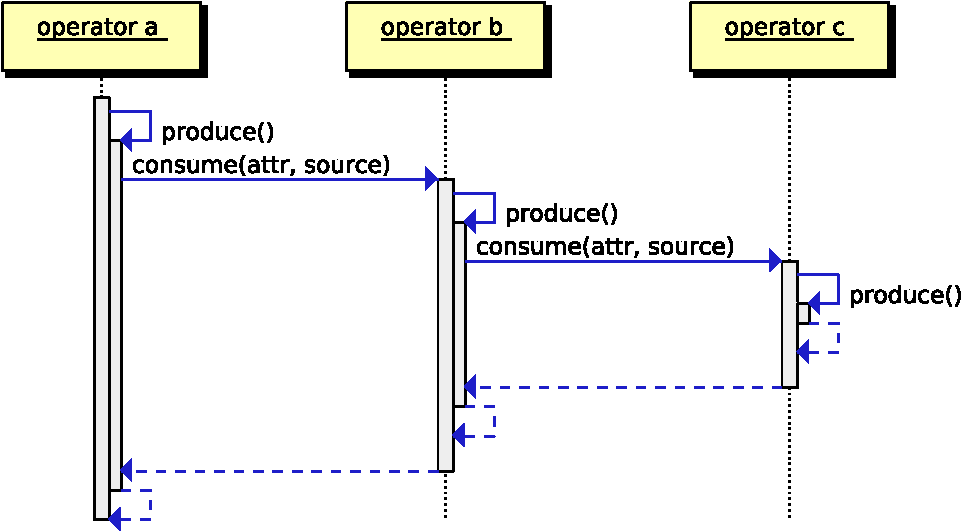
\includegraphics[scale=0.7]{figures/consume_produce}
  }
  \caption[Consume Produce Sequence Diagram]{Consume Produce Sequence Diagram.}\label{fig:consume_produce_sd}
\end{figure}


Therefore, this programming model pushes data towards the next operator, instead of pulling the data. This results in a much better code and data locality. Tuples are pushed from one operator to the next, therefore operators benefit from keeping the data in the CPU registers, which allows very cheap and efficient computation. Only for materializing data memory has to be accessed. Additionally, small code fragments are used to handle large amounts of data in tight loops leading to good code locality and therefore high performance.
\\
These aspects make the execution of operators very fast. Unfortunately, not all operators can be implemented in a way that one tuple gets fully processed before the next one is loaded into the CPU registers. Instead, tuples have to be taken out of the registers and are materialized in main memory for some operators. Those operators break the operator pipeline, therefore we call them~\emph{pipeline breakers}. If an operator materializes all incoming tuples before continuing processing, we call it a~\emph{full pipeline breaker}. An example is a join operator: One side of the two join relations has to be materialized in main memory,  while the other relation is scanned and probed against the materialized data for finding join partners. As the join operator materializes one relation it is a~\emph{pipeline breaker}.
\\
Finally, it is important to note that the \texttt{consume produce} model is just an abstraction layer for the programmer. This abstraction layer is used by the code generation to compile assembly code - within the generated assembly code there is no \texttt{consume produce} present anymore.

\subsection{LLVM Code Compilation}

In this section we discuss the query compilation in greater detail. As in traditional systems, queries are compiled by parsing the query, translating it into algebra and optimizing it. In contrast to a traditional system, the physical algebra is not directly executed, but compiled by the code generation into an imperative program. For generating this imperative program the previously described ~\texttt{consume produce} model is used.
\\
Taking advantage of the structure of the~\texttt{consume produce} model, queries are compiled into native machine code using the LLVM compiler framework~\parencite{LLVM}. LLVM can generate portable assembler code which can be executed directly using an optimizing JIT compiler. With LLVM HyPer uses a very robust assembly code generation, e.g. pitfalls like register allocation are hidden by LLVM. Therefore the assembly code generation is very convenient compared to other compiler frameworks. Furthermore, only the LLVM JIT compiler translates the code into machine dependent code, leading to portable code across computer architectures. Since the LLVM assembler is strongly typed, many bugs can be caught in advance, in contrast to a textual C++ code generation. Furthermore, LLVM produces highly optimized, extremely fast machine code and outperforms in some cases even hand-written code as the assembly language allows code optimization, hardware improvements and other tricks, that are hard to do in a language like C++. All this requires usually only a few milliseconds of compilation time, which is a crucial criterion for database operators with a strong focus on performance.
\\
Additionally, LLVM code is perfectly able to interact with C++, the main language of the HyPer database. Even though LLVM code is robust and convenient to write compared to common assembler code, it is still more painful than writing code in a high-level language such as C++. An interaction of the two languages allows us to implement complex structures in C++ and to reuse existing database logic such as index structures. 
\\
Therefore algorithms can be written in C++ and connected together by LLVM code, where the C++ code is pre-compiled and the LLVM code is compiled at runtime dynamically. An example is the Sort operator: The \texttt{compare} function, comparing two tuples by the rules of a sort query is dynamically generated in LLVM code, depending on the schema of the database. As actual sort function, the built-in C++ \texttt{sort} can be used. This is a great example of the mixed execution model using C++ and LLVM code in one operator.
\\
However, even though C++ and LLVM can both be used implementing an operator, LLVM code is dominant and C++ code should be seen as convenience. For performance reasons it is important that the code executed for most of the tuples is generated code, even though calling C++ from time to time is acceptable. As already mentioned, staying in LLVM allows us to keep the data in the CPU registers and is therefore the preferable way of executing a query. Calling an external function spills all registers to memory, which can be a bottleneck when doing this for all tuples in a big data set.
\\
In conclusion, we have presented the HyPer~\texttt{consume produce} programming model which allows operators to push data towards the next operator in an efficient manner. Furthermore, the LLVM compiler framework with its benefits is introduced used for code generation and interacting with C++ code at runtime. 
This cooperation of LLVM and C++ code regarding programmer friendliness and execution time is one of the dominant patterns in Section~\ref{section:serial_implementation}, where two alternative implementations of the k-Means operator are presented and discussed. 


\section{Requirements and Constraints}\label{section:constraint}
Before discussing the technical implementation details of the k-Means operator, we introduce the requirements and constraints. Obviously, the k-Means algorithm must be implemented as a HyPer operator. That means, the \texttt{consume produce} programming model and the code generation with C++ and LLVM have to be used. The advantage of implementing k-Means as an operator is that it can be used in combination with existing SQL operators, useful for data mining as well, such as grouping and aggregation.
\\
Regarding the functional aspects, the operator must be able to be executed in serial and in parallel, to make use of the computing power of modern database hardware.
\\
As input parameter, the user can specify the number of maximum iterations of the algorithm. If this parameter is omitted, the algorithm runs until convergence. For big data sets this is often a performance problem when only a few data points are changing, but still all the distances have to be computed all over again. Often the result is already accurate enough after a specific number of iterations. Apart from an advantage regarding the running time it is also useful to specify the number of iterations for experiments and evaluation, as we see in Chapter~\ref{chapter:evaluation}.
\\
Further parameters are the initialization strategy and a verbose option. As initialization strategy, the user can select between random initialization and the k-Means++ initialization, as described in Section~\ref{section:kmeans_init}. As default output, an additional column is added to each data row presenting the cluster identifier of the data tuple as an integer. If the verbose option is active, statistics of the run are printed to the console. This information contains the number of iterations, the final center coordinates, the number of assigned data points per center and the squared error sum. 
\\
The number of iterations is crucial for comparing the running time of different k-Means algorithms in a fair manner. It is possible that one execution of the algorithm converges after three iterations, while another one converges after seven iterations, since the number of iterations is non-deterministic due to the random initialization strategy. For fair evaluation, the time per iterations is therefore a good quality measurement and will be used in the evaluation in Chapter~\ref{chapter:evaluation}.


\section{Data Materialization}

\begin{figure}[htsb]
  \centerline{
      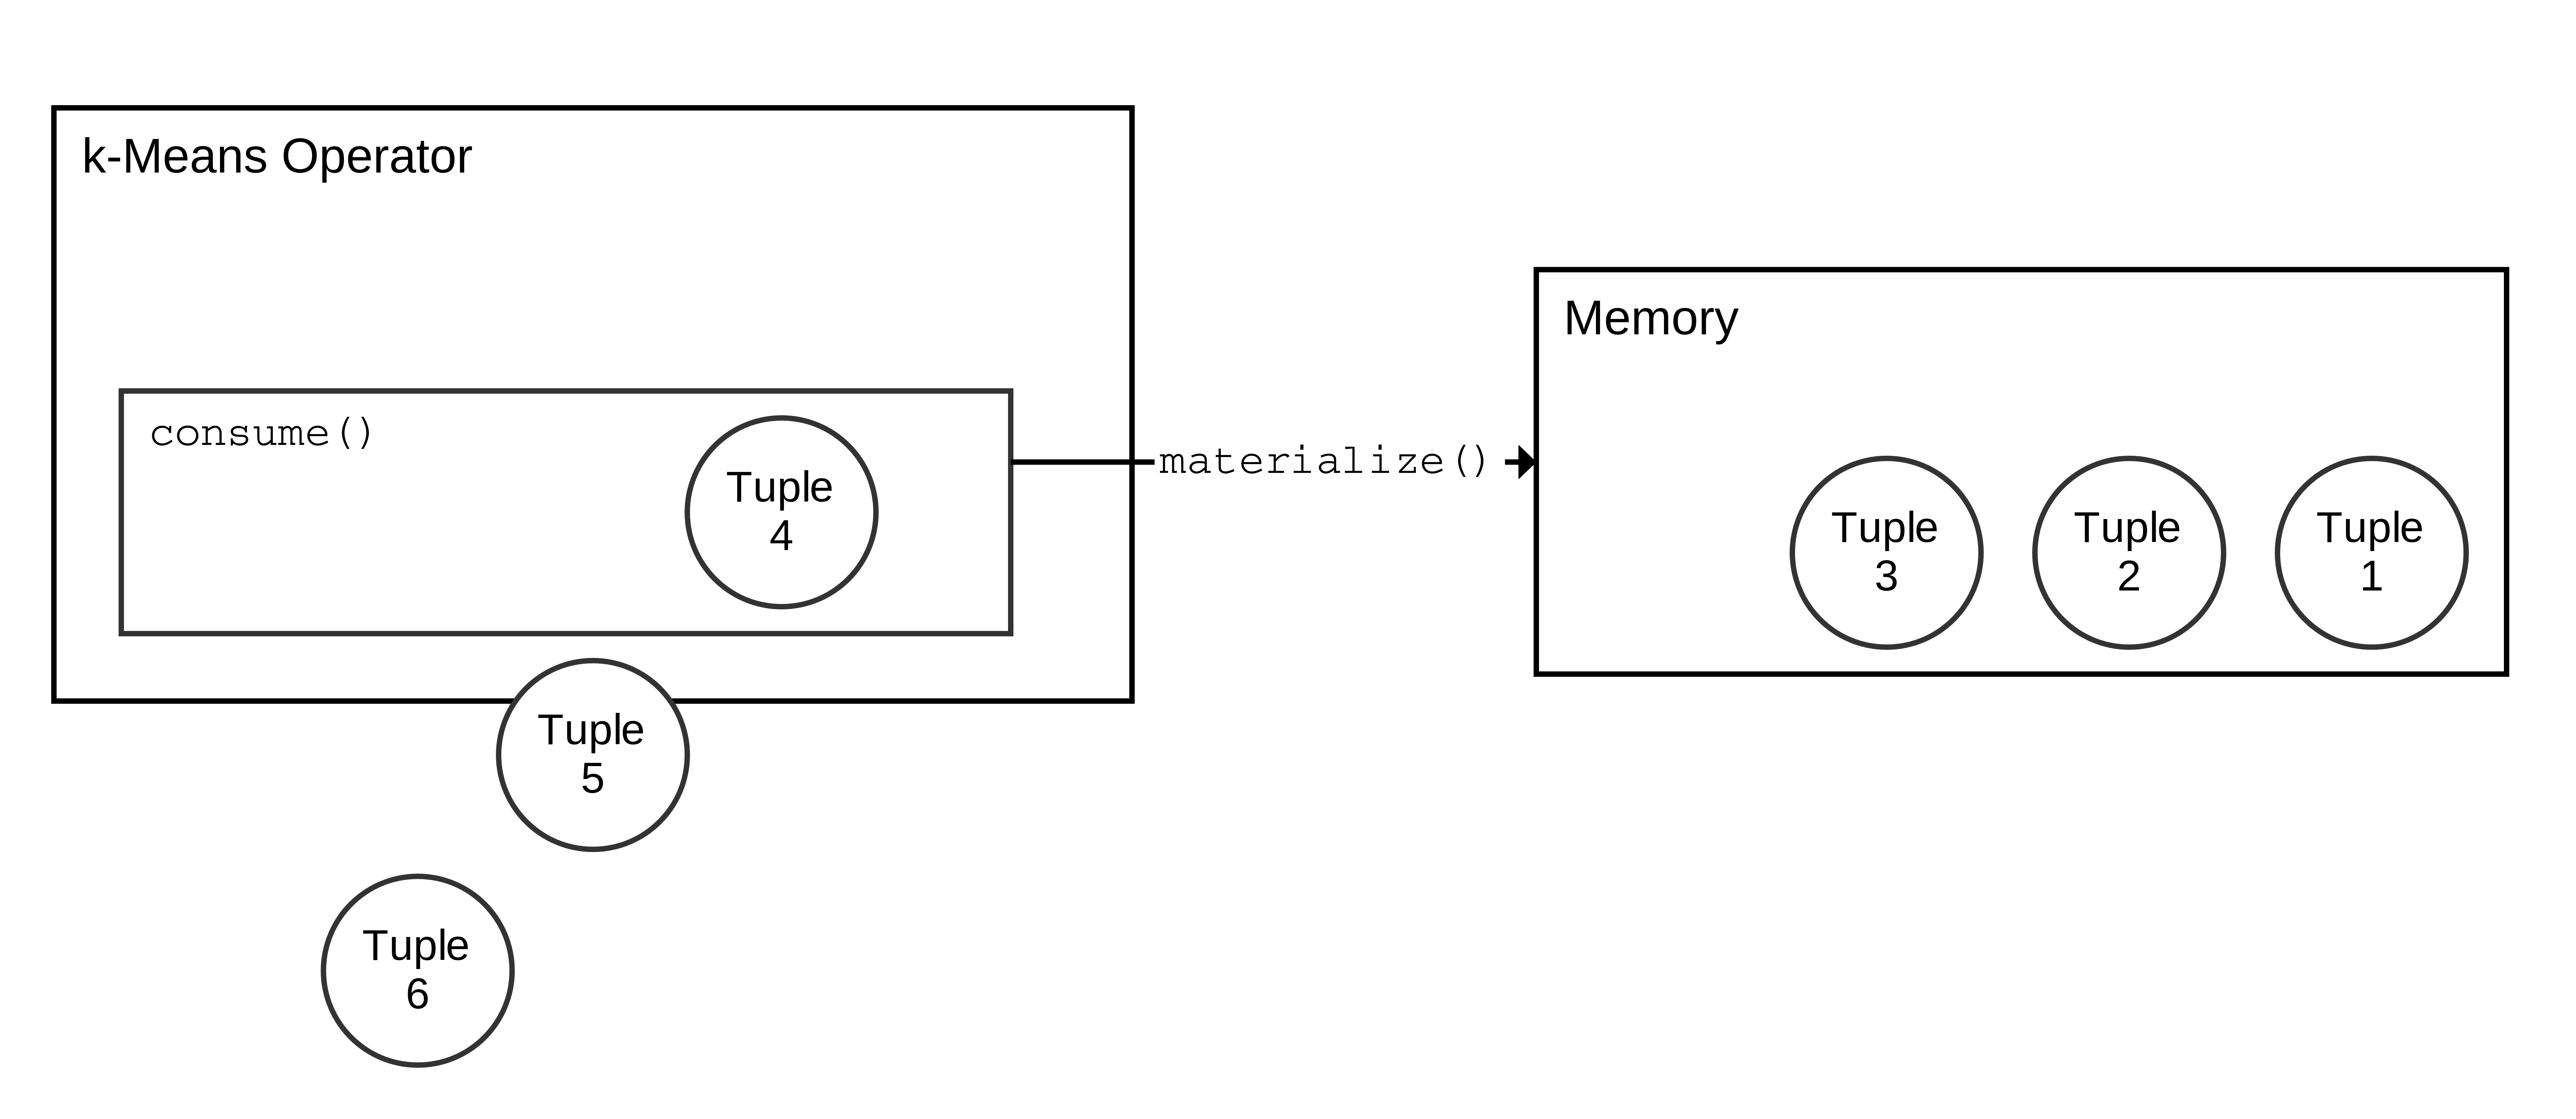
\includegraphics[scale=0.05]{figures/mat1_font2}
  }
  \caption[Data Materialization of Incoming Tuples]{Data Materialization of Incoming Tuples.}
  \label{fig:mat1}
\end{figure}



In this section we discuss the data materialization of the k-Means operator. As already mentioned, materialization is the process of taking incoming tuples out of the CPU registers and write them into memory. Since this decreases the performance of the database, HyPer tries to avoid it, and instead keeps the data in the pipeline as long as possible, i.e. until a~\emph{pipeline breaker} occurs. Unfortunately, k-Means is a~\emph{pipeline breaker}, e.g. center tuples have to be compared with all data tuples to find the minimum distance between them. Therefore, we have to put all tuples into memory. This is depicted in~\autoref{fig:mat1}: Each incoming tuple will be written into main memory when entering the~\texttt{consume} function. 

\begin{figure}[htsb]
  \centerline{
  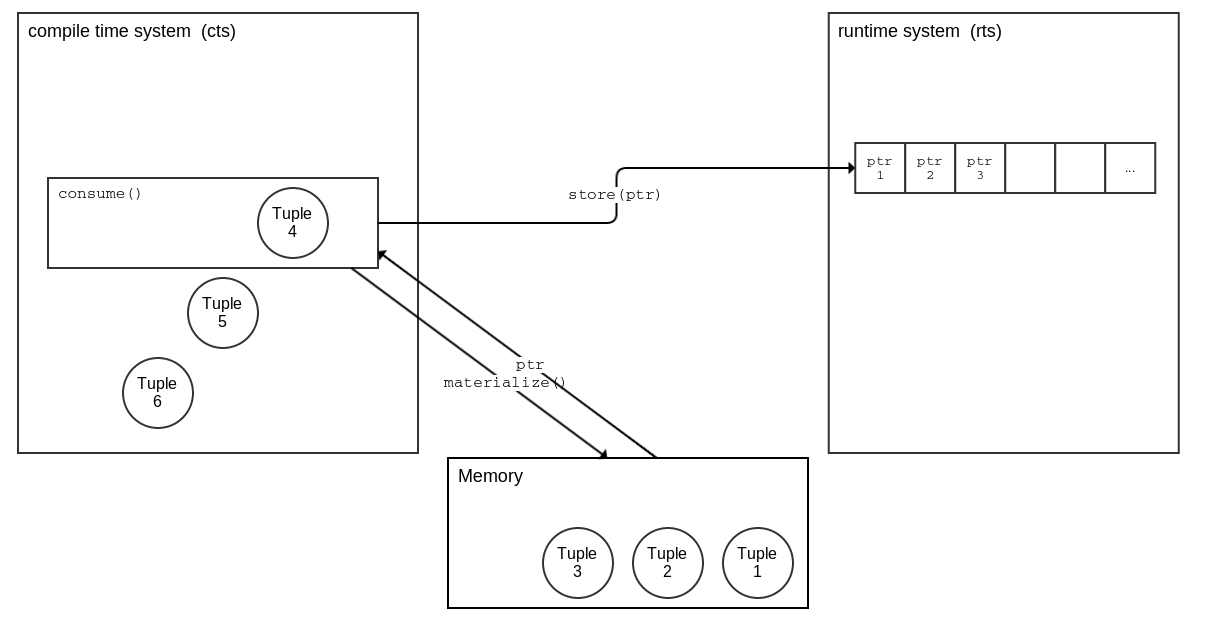
\includegraphics[scale=0.37]{figures/mat2_font4}
  }
  \caption[Data Materialization using the Runtime and Compile Time System]{Data Materialization using the Runtime and Compile Time System.}
  \label{fig:mat2}
\end{figure}

\FloatBarrier

\begin{figure}[htsb]
  \centerline{
  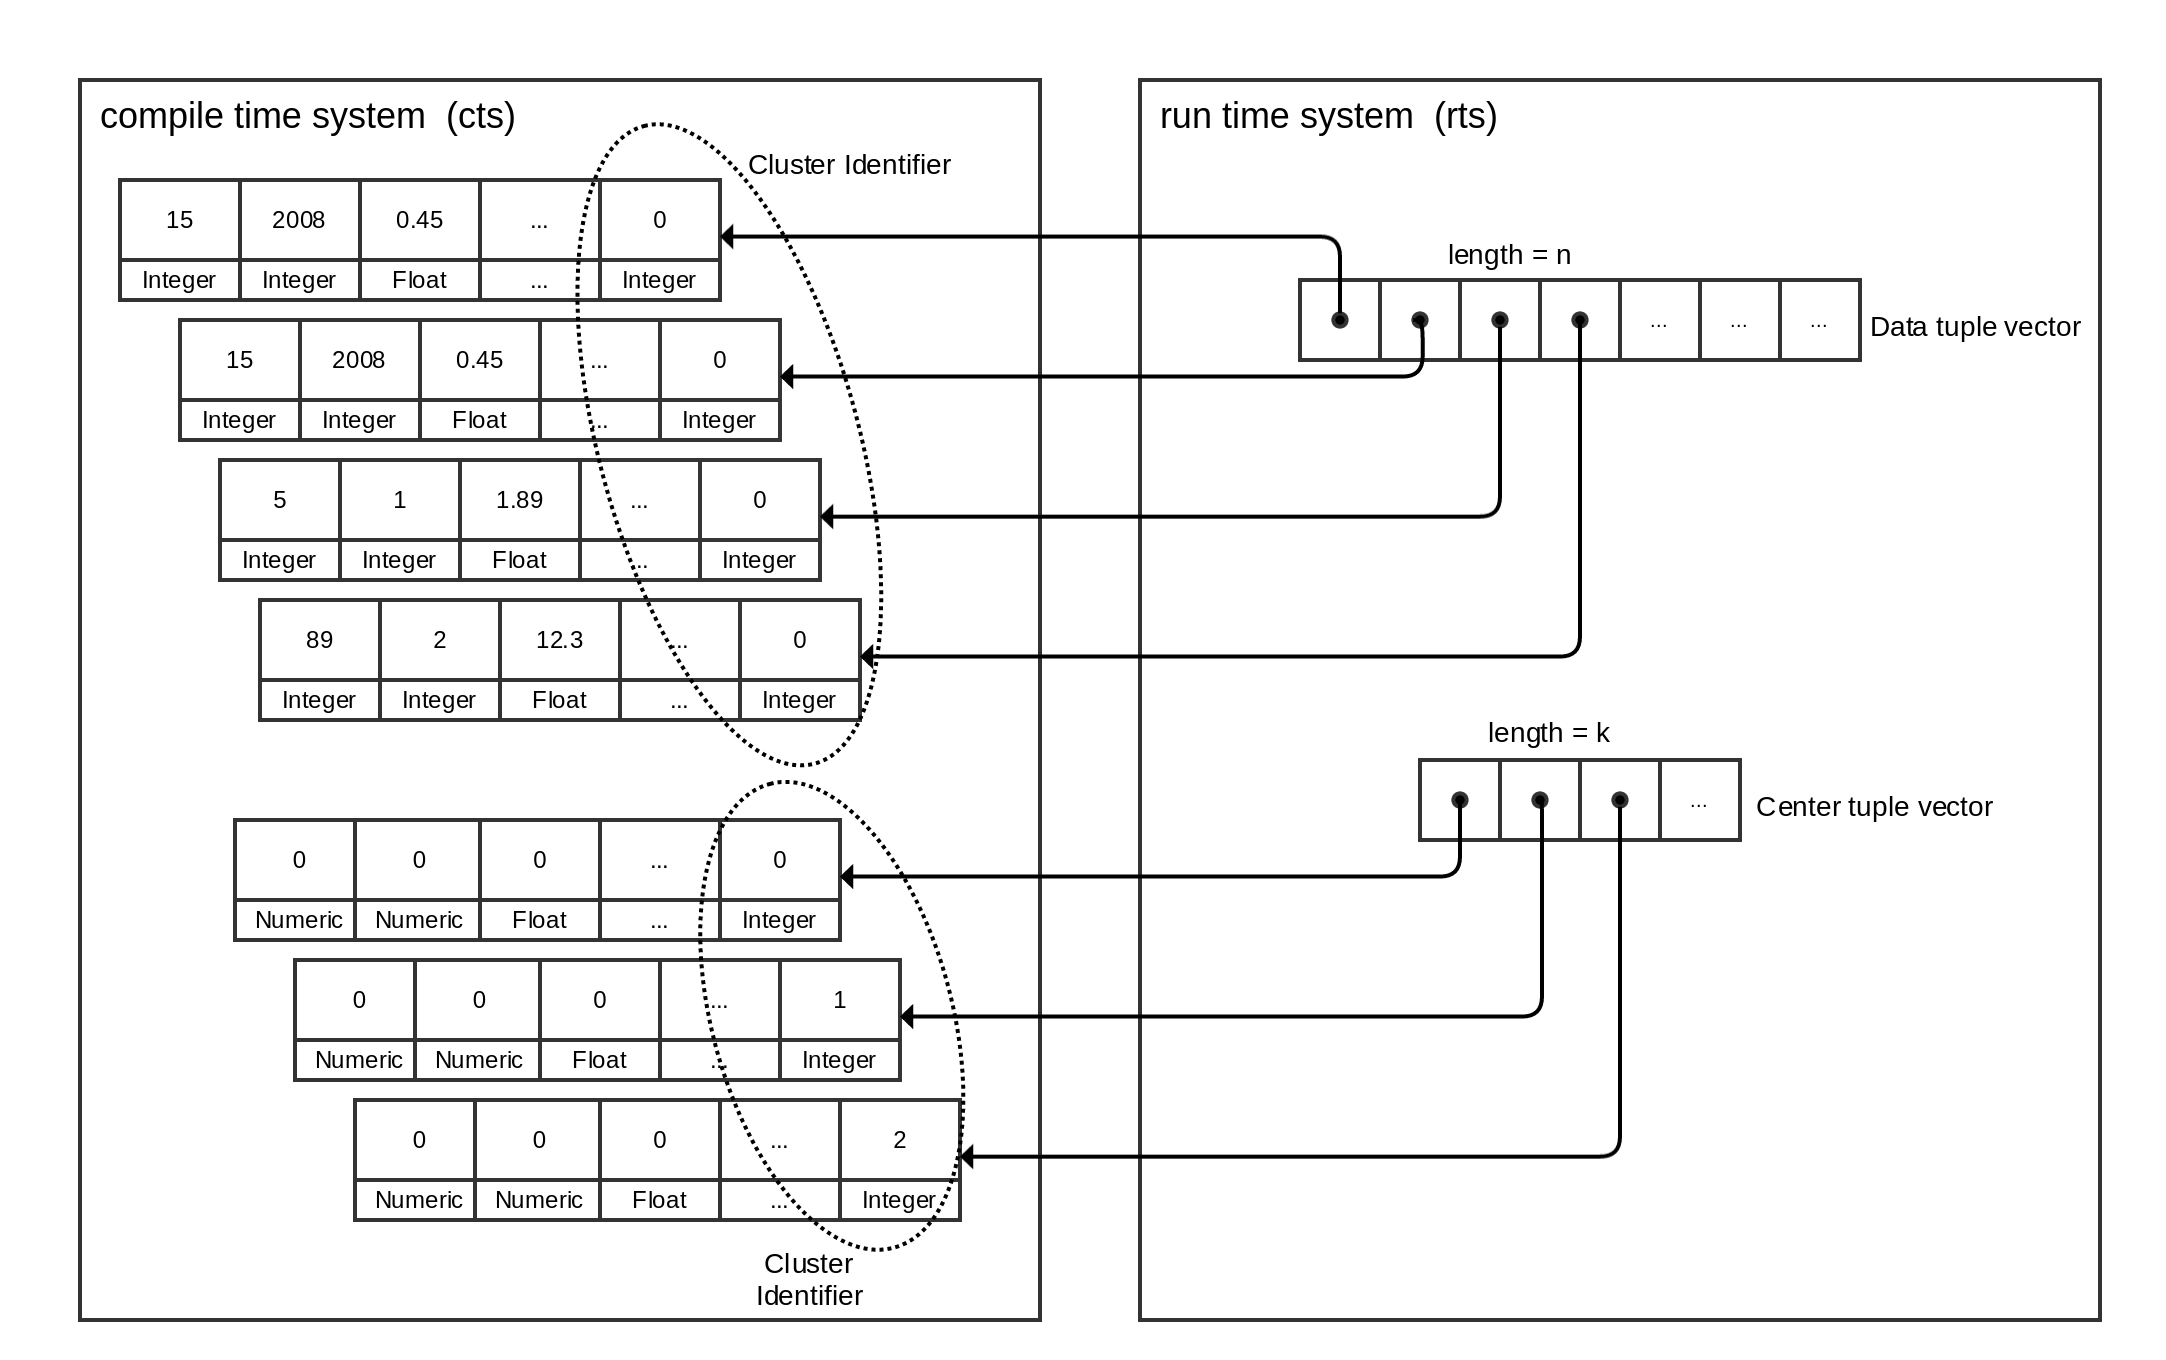
\includegraphics[scale=0.215]{figures/mat3_font2}}
  \caption[The k-Means Data Materialization in Detail]{The k-Means Data Materialization in Detail.}
  \label{fig:mat3}
\end{figure}






This is implemented by using a combination of LLVM and C++ code. In HyPer, LLVM code resides in the \texttt{compile time system (cts)} while C++ resides in the \texttt{runtime system (rts)}. Since the \texttt{compile time system} is the entry point of an operator, the \texttt{consume} function is called and generates code for each tuple. This generated code is materializing the incoming tuples. A pointer to the materialized chunk of memory is then stored in a C++ vector in the \texttt{runtime system}.~\autoref{fig:mat2} depicts this process: Each tuple is materialized into memory by the \texttt{cts} and can be referenced by a pointer stored in a vector in the \texttt{rts}. This vector can later be used to loop through the entire data set: First by looping through the vector in the~\texttt{rts}, getting the pointer to the memory location, which can then be used to load the tuple from memory into the CPU registers in the \texttt{cts}. 


For k-Means it is not enough to store only the data tuples. We also need to reserve memory space for the centers. We do this by materializing the first \texttt{k} tuples of the data set two times: Once as storage for data tuples and once as storage for center tuples. Therefore we have two vectors in the \texttt{runtime system}: One for data tuples of length \texttt{n}, and one for centers of length \texttt{k}. This data materialization for k-Means is depicted in ~\autoref{fig:mat3}.
\\ 
At this point of the process, all data tuples and centers are materialized and an additional field has been added to all of them: A cluster identifier of type integer. For the center tuples, this field stores the center identifier, which goes from 0 to $k - 1$. For data tuples, this field specifies to which center and therefore to which cluster a data tuple belongs to. Initially, all data tuples are assigned to the center with identifier 0. 
\\
Another difference is the cast of data types between data and center tuples. While the data types of data tuples are specified by the table schema, the data types of the center tuples are determined differently since the center is the mean of all the data tuples assigned to that center. Therefore, an integer data value is stored as a numeric data type as center value. Numeric is an exact-value data type for integer and decimal types, and therefore able to store the mean of integer data tuple values. For each data type there exists a rule to cast the respective type from data to center tuple.


\FloatBarrier

\section{Serial Implementation}\label{section:serial_implementation}

After acquiring a basic understanding of HyPer’s operator model, in particular about the interaction of dynamically generated LLVM code and pre-compiled C++ code, we can discuss the actual implementation of a serial k-Means algorithm. The most interesting part of implementing a data mining operator like k-Means in HyPer is the decision of the design of the algorithm, i.e. which parts of the code should reside in the \texttt{compile time system} and which parts in the \texttt{runtime system}. 
\\
This question is not trivial because there are no strict rules and several possibilities. For example, a dynamic generation of code works best for comparing tuples with each other as in the sort operator, or the computation of a distance in the k-Means operator. This code has to handle different data types depending on the table schema and therefore generated code is preferable. For other parts, like the implementation of a sort function or the combination of loops in k-Means, it is not so obvious where to put the code.
\\
In this work we present two different ways of implementing a serial k-Means operator in HyPer, first by implementing the algorithm in C++ with only a few generated LLVM functions, e.g. to compute the distance. Then, a system is presented implementing k-Means almost entirely in LLVM. Only small parts, like initializing the random centers are implemented in C++. This implementation benefits of generated, compact code and we expect performance gains over the C++ driven implementation.


\subsection{A C++ driven Implementation}

As first implementation approach we present a C++ driven version. The term C++ driven is maybe misleading, since all operators start their main computation after invoking their \texttt{consume} function, which is an LLVM generated function. Even though the operator starts working in the \texttt{compile time system}, in this implementation, \texttt{cts} calls the k-Means operator of the \texttt{runtime system} and gives the full control to the C++ code, until the k-Means algorithm terminates. 

~\autoref{fig:cpp_driven} shows this interaction in a sequence diagram: The algorithm is invoked in the \texttt{compile time system} and calls the k-Means function of the \texttt{runtime system}. The entire execution stays now in the \texttt{runtime system}, with calls back to the~\texttt{cts} from time to time, but immediately returns to the~\texttt{rts} once a function call terminates. 
\\
At first, the centers are selected. Let’s assume we are using a random initialization strategy. \texttt{K} times, a random pointer of the data vector is selected, and its values are copied to the corresponding center tuple. Therefore, the \texttt{centerPtr} and the randomly selected \texttt{dataPtr} are parameters of a generated \texttt{setCenter} function. This function loads both tuples from memory using its corresponding pointers. Next, the data values are casted if necessary, since we have different data types among center tuples and data tuples as described in the previous section, and then copied to the center tuple. Afterwards, the center tuple is written back to memory. This process is repeated until all $k$ centers are determined.

\begin{figure}[htsb]
  \centering
  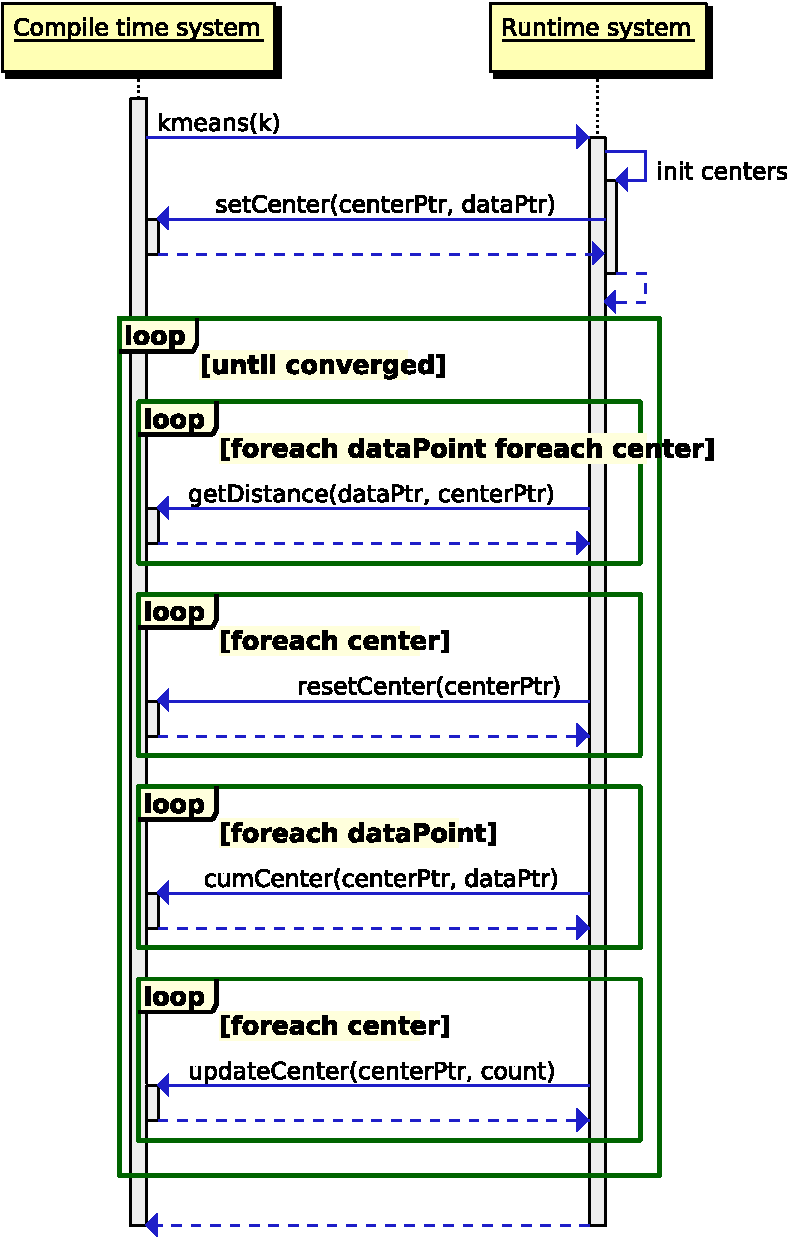
\includegraphics[scale=0.55]{figures/cpp_driven}
  \caption[The k-Means Algorithm - C++ driven]{The k-Means Algorithm - C++ driven.}
  \label{fig:cpp_driven}
\end{figure}

After selecting the initial set of centers, the \texttt{runtime system} starts its outer loop, running until k-Means converges. In the outer loop, the \texttt{runtime system} calls the \texttt{compile time system} to compute the distances between all data points and center points to find the closest center for each data tuple. Therefore, \texttt{getDistance} is invoked for each \texttt{dataPtr} - \texttt{centerPtr} combination. The closest center for each data point is then stored in an \texttt{unordered\_map} in C++ for efficient lookup. 
\\
After finding the closest center for each data tuple, the centers have to be updated. Since the materialization of centers is done in LLVM code, the \texttt{runtime system} has to call the \texttt{compile time system} again, in fact several times: First, a \texttt{resetCenter} function is called for all center pointers to set the center values of the center tuples to zero. Then, the new mean can be computed. 
\\
The computation of the mean is done in two steps. First, the data points are accumulated for each center, and then divided by the number of data points belonging to each center. This simple mean computation leads to several \texttt{compile time system} calls for our algorithm. For each data point, its values are added to the center tuple it belongs to. Therefore, the \texttt{cumCenter} function is called, adding the values of the data point to the center point and also updating the cluster identifier of the data tuple. The \texttt{runtime system} keeps track of how many tuples are added to each center. When finished, each center is called again to compute the actual mean of the center dividing by the count of data tuples assigned to the center using the \texttt{updateCenter} function. This concludes the first iteration of the algorithm. The next iteration starts then again with the computation of the closest center for the data points. This process continues until the algorithm converges.
\\
Using this implementation approach the main control of the algorithm remains in the \texttt{runtime system}. However, this kind of implementation leads to many calls between the \texttt{compile time} and the \texttt{runtime system}, in total $(n+2) \cdot k + n$ calls per iteration, as ~\autoref{tab:llvm_calls} shows. The next section presents an implementation that prevents the algorithm from too many calls between the two systems, which might affect the performance of the operator in a beneficial way.




\begin{table}[htsb]
  \caption[LLVM number of calls]{Generated Function Calls per Iteration.}\label{tab:llvm_calls}
  \centering
  \begin{tabular}{l l}
    \toprule
      Generated Function & Calls per Iteration \\
    \midrule
      \texttt{getDistance} & $k \cdot n$ \\
      \texttt{resetCenter} & $k$ \\
      \texttt{cumCenter} & $n$ \\
      \texttt{updateCenter} & $k$ \\
    \bottomrule
      Total & $k \cdot n + k + n + k = (n + 2) \cdot k + n$ \\
  \end{tabular}
\end{table}


\subsection{An LLVM driven Implementation}

As already stated, LLVM code generation encourages the interaction between LLVM and C++ code which is exploited a lot in the C++ driven implementation of k-Means: The algorithm is implemented in C++ and benefits from high-level data structures such as \texttt{unordered\_maps} and the convenience of the C++ syntax, allowing a quick implementation. 
\\
However, the approach presented in the previous section leads to many calls between the \texttt{compile time} and the \texttt{runtime system}, as shown in ~\autoref{tab:llvm_calls}, which could possibly affect the performance of the operator. Therefore, a second approach has been explored, implementing the k-Means algorithm almost entirely in LLVM code. Only the random initialization of the center points remains in C++. When thinking about such an implementation, we have to be aware that we cannot use C++ high-level data structures anymore, but have to work with what LLVM gives us.


\begin{figure}[htsb]
  \centerline{
    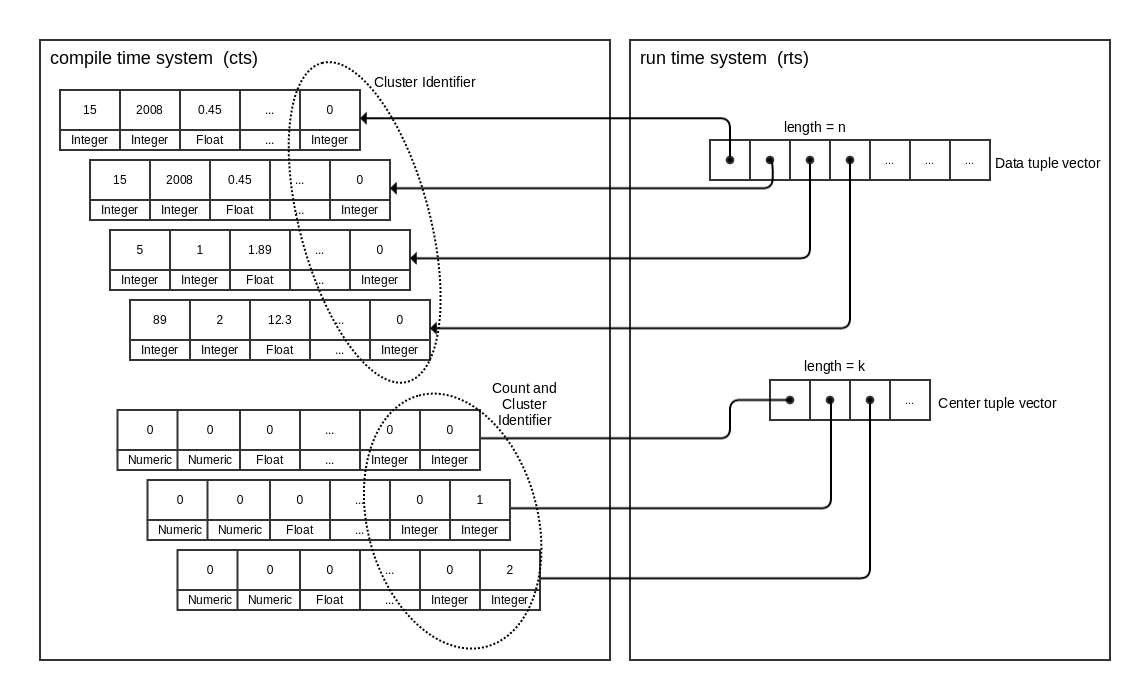
\includegraphics[scale=0.4]{figures/mat4_font}
  }
  \caption[The k-Means Data Materialization - LLVM Implementation]{The k-Means Data Materialization - LLVM Implementation.}
  \label{fig:mat4}
\end{figure}

The only data structure we have used so far in LLVM was a structure to materialize the data and center tuples. In order to keep things simple, we exploit this data structure even further to use it with the LLVM k-Means implementation, without using any other data structures in addition.
So the question is: How do we extend the existing data structure of the \texttt{compile time system} to emulate the C++ code we want to omit? This can be done by extending the center data structure when materializing the centers in the \texttt{consume} function. As ~\autoref{fig:mat4} shows, an additional field has been added to the center tuple to keep track of the count, determining how many data points are close to this center. With this small modification we can implement our algorithm in LLVM with the use of only one data structure.
\\
The LLVM driven algorithm is depicted in a sequence diagram in ~\autoref{fig:llvm_driven} and shows the indirection of the calls compared to the sequence diagram of the C++ driven approach in ~\autoref{fig:cpp_driven}: This time, the LLVM code executes the algorithm, calling C++ code from time to time. There are also no loops around the calls between the LLVM and C++ code, therefore the number of calls is very low. 
\\
As in the previous implementation, the algorithm starts with selecting the random centers. This process does not change, but afterwards the control of the algorithm goes back to the~\texttt{compile time system}. The only information the~\texttt{compile time system} requires from the~\texttt{runtime system} is the first pointer and the last pointer of the data vector and of the center vector, respectively. Then, the~\texttt{compile time system} is ready to execute the k-Means algorithm without any further interaction with the~\texttt{runtime system}. 
\\
Next, the minimum distances are computed between center and data tuples. The distance function was already implemented in LLVM code for the C++ driven approach and the code can be reused, only the loops around the \texttt{getDistance} function have to be implemented in LLVM. 
\\
The next step is to update the center tuples. The functionality of the \texttt{resetCenter} function can be kept the same, as well as the \texttt{cumCenter} function. Again, the loops around the functions are now implemented in generated LLVM code. When computing the mean of a center, we have to keep track of the count. For that purpose we are using the additional field of each center tuple created on data materialization. Whenever we are adding data tuples to the corresponding center, we increment the count. When invoking the \texttt{updateCenter} function, this count is used to compute the mean using a division. 



\begin{figure}[htsb]
  \centering
  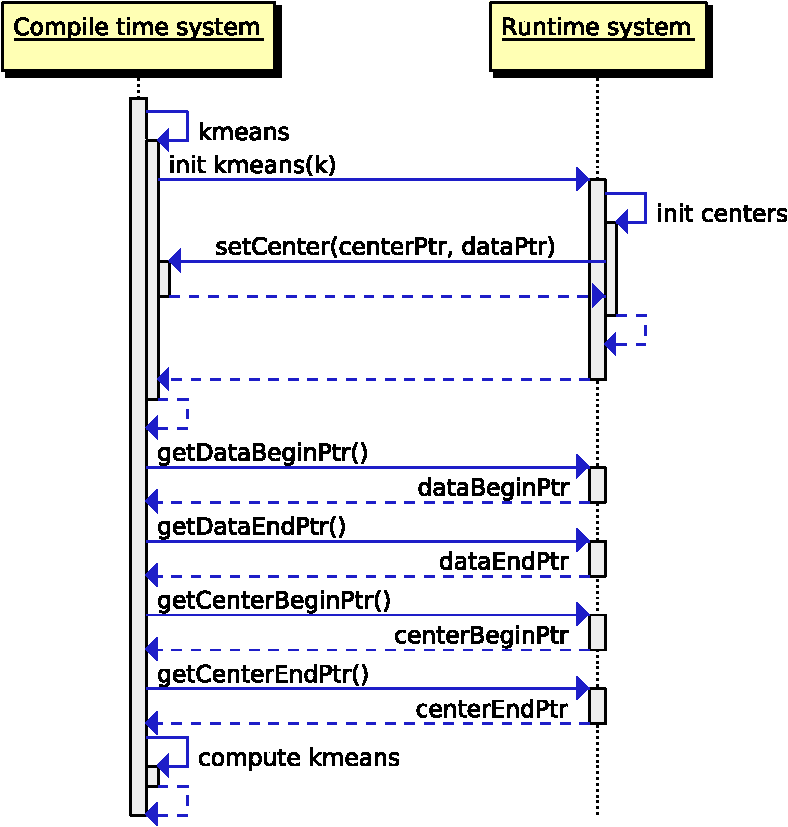
\includegraphics[scale=0.55]{figures/llvm_driven}
  \caption[The k-Means Algorithm - LLVM driven]{The k-Means Algorithm - LLVM driven.}
  \label{fig:llvm_driven}
\end{figure}



Even though the difference between the two presented approaches does not seem to be huge since the overall programming concept remains the same, the difference in the code is significant. In particular using LLVM over high-level C++ constructs adds an overhead in the number of code lines. Therefore, the LLVM code in the second approach is harder to understand and to maintain. On the other hand, while the C++ version has $(n + 2) \cdot k + n$ calls from the~\texttt{runtime} to the~\texttt{compile time system} per iteration, the LLVM version has no calls at all during the execution of the algorithm. Instead, it only requires the first and last pointer of the data and center vector at the beginning of the algorithm. This leads to performance improvements as we see in Chapter~\ref{chapter:evaluation}, where the LLVM driven approach shows better results for all carried out experiments.


\subsection{Initialization Strategy}\label{sub:init}

In the so far discussed implementation details of the k-Means algorithm we assumed to use a simple random initialization strategy. Such a strategy can be implemented in the~\texttt{runtime system}, since only C++ code is used for finding a random subset of length \texttt{k} of the data tuples, which can be implemented using the Fisher-Yates shuffle algorithm~\parencite{fisheryates}. 
\\
However, in Section~\ref{section:kmeans_init} we figured out that one of the most popular variations of k-Means is k-Means++. The k-Means++ algorithm uses an extended initialization strategy by choosing data points as center point with higher probability the further away they are from the already chosen set of center points. Often, this leads to improvements in both speed and quality of the clustering.
\\
For implementation this means that we have to compute the distance from the chosen center points to the data points in the initialization phase too. This can be done very conveniently for the C++ version, as the \texttt{getDistance} function is implemented already. Therefore, the main initialization routine can be written in C++, only the \texttt{getDistance} function is used as generated function.
\\
For the LLVM version, we still keep the center initialization in the \texttt{runtime system} to benefit of high-level C++ program structures. To realize the k-Means++ algorithm, we have to add an explicitly generated \texttt{getDistance} function to the LLVM code: Even though the LLVM version computes the distance as well, there is no generated function anymore, since the distance generation is part of the generated program. Once we have added this function, k-Means++ can be implemented the same way as in the C++ driven approach.

\section{Parallel k-Means}\label{section:parallel_implementation}

After presenting two single-threaded implementations of the k-Means algorithm, in this section we show an approach to implement k-Means in HyPer in a parallel way to make use of all cores. Keeping in mind that HyPer is a high-performance database system written in C++, it makes already excessive use of multi-threaded programs, therefore it is only logical to add a parallel version of k-Means too. In the following we use the serial C++ version and modify it to allow parallelism. The C++ version is used over the LLVM version due to higher maintainability, readability and the limited time of this work.
\\
The main bottleneck of the serial implementation is to compute the closest center for each data point: The algorithm has to calculate the distance to each center point which has to be performed in each iteration. This means $k \cdot n$ independent distance computations, which can benefit a lot from parallelism and a computation in independent threads.
\\
When executing a HyPer operator in parallel, the~\texttt{consume} function is called for chunks of input tuples instead of the entire data set. Consider a system with four threads as shown in~\autoref{fig:parallel}: Each thread consumes one fourth of the data set and materializes the input tuples. Also in the~\texttt{runtime system}, there are now vectors for each thread, storing the pointers to the input tuples. 


\begin{figure}[htsb]
  \centerline{
    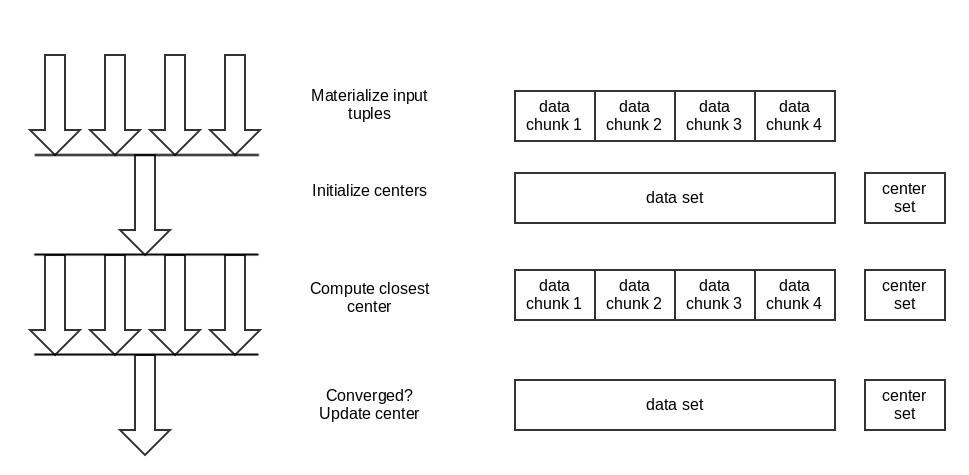
\includegraphics[scale=0.4]{figures/parallel_font}
  }
  \caption[The k-Means Algorithm as Parallel Operator]{The k-Means Algorithm as Parallel Operator.}
  \label{fig:parallel}
\end{figure}

After consuming the data the k-Means algorithm continues with choosing the initial center set. For that, we have to break with the parallelism: For a random initialization of the clusters, center tuples are selected from the entire data set randomly. This is even more important for the k-Means++ initialization strategy computing centers regarding a distance function. While we could select random data points for the center just from one data chunk, this is not possible anymore for the advanced logic of the k-Means++ initialization strategy. Therefore, we create a global vector storing pointers to all materialization tuples. Now we can select the global center points using one of our initialization strategies and continue the parallel program sequence afterwards.
\\
After this serial initialization we can continue the parallel execution of the algorithm and compute the distance from each data point to each center point. This expensive computation can be done independently in each data chunk on a separate thread and benefits from the potentials of parallelism. Ideally, this leads to a running time advantage of one fourth of the serial execution, however, due to the overhead of process creation and management we will not be quite able to attain such high improvements, as the experiments in Chapter~\ref{chapter:evaluation} show.
\\
After this parallel computation, we jump back to a serial execution mode and check for each thread if the program has converged. Only if all threads have converged, we can terminate the algorithm and output the result of the clustering. Otherwise, we update the center points by the newly assigned data points. In the first version of this parallel implementation, this step is done in serial as already presented in Section~\ref{section:serial_implementation}. However, here is potential for parallelizing the program even more, which is a goal for future implementations as we see in Chapter~\ref{chapter:conclusion}.
\\
In the evaluation chapter we compare the parallel k-Means algorithm with the two serial implementations. Even though only one part of the algorithm is parallelized and with the overhead of introducing the parallelism in mind, we expect huge performance gains since the parallelized code part contains many independent computations well-suited for multi-threaded execution.






\chapter{Evaluation}\label{chapter:evaluation}

In this chapter we provide an extensive experimental evaluation of the HyPer k-Means operator and compare the different HyPer implementations to each other as well as to some of the state-of-the-art clustering tools presented in Chapter~\ref{chapter:related}. All experiments have been performed on a workstation equipped with sixteen 2.93 GHz CPUs and 64 MB of main memory.


\section{Data Sets}
As objective comparison criterion the execution time per iteration is measured in the following experiments, as described in Section~\ref{section:constraint}. Therefore the different technologies can be compared in a fair way and random initialization and internal improvements for faster convergence do not affect the outcome. For the experiments a real world data set is used and four synthetic data sets have been generated\footnote{The data set generation script can be found in Appendix~\ref{appendix:generator}.}. The synthetic data sets are chosen in a way that both the number of instances and the number of dimensions are varying, covering many real world use cases and also allow a reasonable comparison between the data sets. The used data sets are shown in~\autoref{tab:dataset}.

\begin{table}[htsb]
  \caption[The Data Sets]{The Data Sets.}\label{tab:dataset}
  \centering
  \begin{tabular}{l l l l l}
    \toprule
      & Instances & Dimensions & Size (byte) & Size (Gigabyte) \\
    \midrule
      3D Network        & 434,874    & 4     & 20,673,913 & 0.019 \\
      High Dimensional  & 50,000     & 50    & 10,000,000 & 0.009 \\
      Medium Size       & 15M       & 4     & 240,000,000 & 0.22 \\
      Medium Size HD    & 15M       & 50    & 3,000,000,000 & 2.79 \\
      Large Size        & 150M      & 10    & 6,000,000,000 & 5.59 \\
    \bottomrule
  \end{tabular}
\end{table}



\begin{itemize} 
\item 3D Network: The first data set contains the 3D spatial road network data of a road network in North Jutland, Denmark~\parencite{3dnet}. It is a real world data set available at the UCI Machine Learning Repository~\parencite{frank2010uci} and consists of 434,874 data points in four dimensions: The id of the road segment, the latitude, the longitude and the altitude of the segment. The id is a large integer, the other dimensions are floating point numbers. The size of the data set is 19.72 MB, therefore it is a rather small data set.

\item High Dimensional: As second data set a synthetic data set with 50,000 data points has been generated. The data set consists of 50 dimensions and is used to resemble a rather small but high dimensional data set. All dimensions are floating point numbers. The size of the data set is 9.50 MB, hence it is even smaller then the network data set.

\item Medium Size: Next, a larger data set has been created to test the tools on millions of tuples: The medium size data set consists of 15 million data points in four dimensions. The size of the data set is 228.88 MB, therefore almost 12 times larger than the network data set.

\item Medium Size High Dimensional (HD): For comparing the previous data set with a high dimensional data set, the medium size high dimensional data set has been generated. As the medium size data set, it consists of 15 million data points, this time in 50 dimension. This leads to a growth from 0.23 GB to 2.79 GB. The same number of instances with different dimensions allows us to evaluate how different algorithms behave when dimensions are growing.

\item Large Size: Finally, we generated an even larger data set. The number of instances has increased by a factor of 10 compared to the medium data set, resulting in 150 million instances. As number of dimensions, 10 has been chosen as a middle way between the previously chosen 4 and 50 dimensions. This leads to a data set of 5.59 GB.
\end{itemize} 

Additionally to varying the data sets, we also vary the cluster number $k$ from 3, 10 and 20 for each data set for each used tool. Since none of the data sets has a natural optimal clustering, there is no perfect $k$, therefore a varying $k$ works best for comparing different tools.


\section{Competitor Systems}

As already described in Chapter \ref{chapter:related}, there exist many software solutions and programming languages for data mining. In this section we look at a subset of the tools implementing the k-Means clustering algorithm and use them for comparison with our own k-Means HyPer operator. To make the results comparable in a fair manner, we only use tools that give enough information about the clustering process, e.g. the number of iterations, the cluster compactness and most importantly, the applied algorithm. Not all tools are implementing the Lloyd algorithm or, as for R, the default algorithm is the Hartigan and Wong algorithm, and the usage of the Lloyd algorithm has to be explicitly specified as an input parameter.
\\
Since k-Means is a non-deterministic algorithm, the number of iterations is the most important criterion to make the results comparable. The running time of k-Means depends almost entirely on the number of iterations the algorithm has to make, which is largely influenced by the non-deterministic initialization. Therefore the running time should be relative to the number of iterations. Unfortunately, neither ELKI's nor SciPy's k-Means implementation provide the number of iterations as output. Therefore, a fair comparison is not possible. Fortunately, Weka, R and Julia provide good configuration possibilities as well as a result set that contains information about the number of iterations. While Weka is written in Java, R and Julia are both written in their own high-level syntax. Even though, critical code parts are implemented in C, C++ and Fortran for better performance. Without the overhead of an entire database system behind, it will be interesting to compare HyPer with Weka, R and Julia.
\\
We are excluding the big data solutions, middleware tools and analytical databases presented in Chapter~\ref{chapter:related}, since these tools are often only applicable for specific use cases, e.g. tremendously large volumes of data, or require specific environments or proprietary software. Instead, we are comparing the HyPer k-Means solution with well-known, open-source clustering tools used by data scientists everyday.
\\
The usability and user experience among R and Julia is very similar: Both can be run as interactive program or as script in their functional language, and both can import the test data sets in csv format. HyPer can be run as interactive console program or as script, too, and provides efficient csv loading~\parencite{hypercsv}. Weka provides a GUI with the Weka Explorer, and can be run from the command line, too, or directly in Java programs. Internally, Weka uses the arff format for its algorithms. Using the Weka GUI to convert the original data (in our case in csv format) into the arff format feels fairly natural, as it happens in a preprocessing step when loading the data. However, when using the command line or Java programs to read a csv file, the file has to be preprocessed to the arff format first by an additional command. This takes time and is not as convenient compared to the other tools.
\\
However, the main reason for not including Weka in the next sections is the disappointing running time compared to Julia, R and HyPer, as depicted in~\autoref{tab:weka_final}. The table shows the median, the 90th and the 95th percentile of the running time per iteration of 100 Weka clusterings for $k = 3, 10$ and $20$. Compared to the other tools, which running time we will present in later sections in detail, Weka performs poorly: On the network data set, Weka is still slower by a factor of 7 compared to Julia's implementation, which is already the slowest tool on that data set. On the high dimensional data set, the HyPer C++ implementation shows the worst results, however, Weka is slower by a factor of around 6. As last test, the medium size data set was run against Weka, and it is slower by a factor of 10 for $k = 3$, 8 for $k = 10$ and 7 for $k = 20$ compared to Julia, the slowest one regarding this data set. Because of this tremendous differences in running time, we stopped the experiments with Weka and decided not to include Weka in the following sections and only compare the performance of the HyPer operator to R and Julia.

\begin{table}[htsb]
  \caption[Weka Results - Time per Iteration]{Weka Results - Time per Iteration in seconds.}
  \label{tab:weka_final}
  \centering
  \begin{tabular}{ll l l l |l l l |l l l }
    \toprule
      &  & \multicolumn{3}{c}{Network 3D} & \multicolumn{3}{c}{High Dimensional} & \multicolumn{3}{c}{Medium Size}  \\
      & \emph{k} & 3 & 10 & 20 & 3 & 10 & 20 & 3 & 10 & 20 \\
    \midrule
      \parbox[t]{2mm}{\multirow{3}{*}{\rotatebox[origin=c]{90}{\emph{percentile}}}} & 50  & 1.39 & 1.54 & 1.93 & 1.08 & 1.39 & 1.90 & 54.01 & 58.25 & 71.11 \\
      & 90  & 1.48 & 1.60 & 2.02 & 1.16 & 1.44 & 1.98 &59.16 & 62.54 & 87.16 \\
      & 95  & 1.49 & 1.61 & 2.06 & 1.19 & 1.46 & 2.01 & 59.79 & 64.31 & 88.54 \\
    \bottomrule
  \end{tabular}
\end{table}



\section{Serial Implementation}\label{section:serial}

In this section we compare the C++ driven and the LLVM driven implementation with each other, both described in detail in Section~\ref{section:serial_implementation}. The experiments differentiate between the compilation and the execution time. The compilation time is the time for generating LLVM code, while the execution time is the time for executing the k-Means algorithm after the LLVM code was generated. Since the compilation time can be seen as a one-time setup time, we expect the execution time to be much larger. 
\\
For each data set, the two HyPer implementations are tested for $k = 3,10$ and 20. For each $k$ the algorithm is executed 100 times with a maximum number of iterations of 10. As result, the median time per iteration in seconds is stated. For better comparability the compilation time is also relative to the number of iterations, even though it stays constant as the number of iterations grows.
\\
~\autoref{tab:network_serial} shows the result of the two serial implementations for the network data set. As we observe the compilation time is independent of the cluster number $k$. Also the compilation time does not differ among the C++ implementation and the LLVM version. In contrast, the execution time increases as the cluster number $k$ increases. This is true for both implementations. 

\begin{table}[htsb]
  \caption[3D Network - Time per Iteration]{3D Network - Time per Iteration.}\label{tab:network_serial}
  \centering
  \begin{tabular}{l l l l l}
    \toprule
      & HyPer C++ & & HyPer LLVM & \\
      k & compilation[s] & execution[s] & compilation[s] & execution[s] \\
    \midrule
      3 & 0.0050 & 0.0680 & 0.0046 & 0.0171 \\
      10 & 0.0044 & 0.0947 & 0.0046 & 0.0502 \\
      20 & 0.0045 & 0.1391 & 0.0046 & 0.0901 \\
    \bottomrule
  \end{tabular}
\end{table}


For better visualization, ~\autoref{fig:hyper_network} depicts the same result as stacked bar charts. Again we observe that the compilation time is low and constant, while the execution time differs among the implementations. For $k = 3$, the execution time of the C++ version is almost four times the execution time of the LLVM version. For $k = 10$ it is two times the execution time and for $k = 20$ it is 1.5 times, respectively. On the other hand that means that for a larger cluster number $k$, the LLVM execution time grows  faster than the execution time of the C++ version. Actually, from $k = 3$ to $k = 10$, the LLVM version grows by a factor of 2.9, while the C++ version grows by 1.4. From $k = 3$ to $k = 20$ the growth is even more significant, from factor 2 for the C++ version to 5.3 for the LLVM version.


\begin{figure}[htsb]
  \centering
  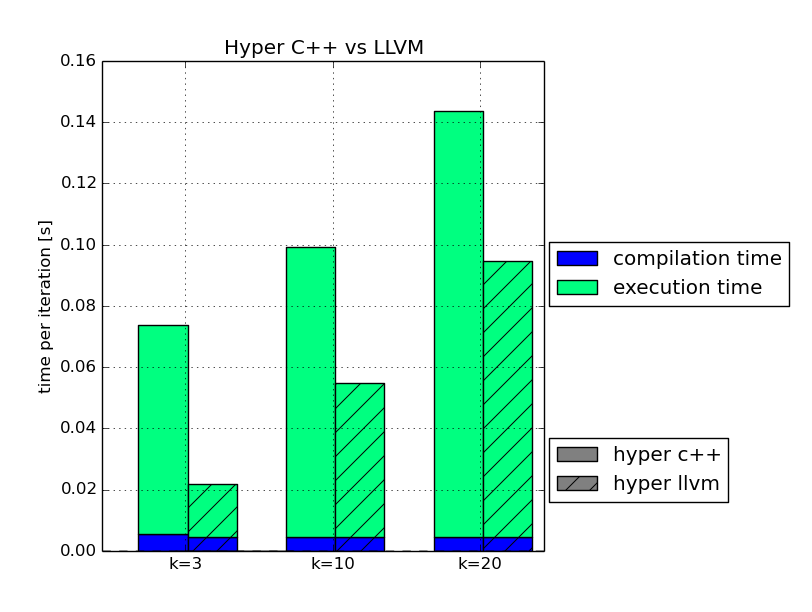
\includegraphics[scale=0.5, trim="0cm 1.5cm 0cm 0cm"]{figures/charts/hyper_network}
  \caption[3D Network - Time per Iteration]{3D Network - Time per Iteration.}
  \label{fig:hyper_network}
\end{figure}

This gives us the first interesting results. Although the C++ version is implementing k-Means using LLVM only for generated functions, the compilation time does not differ compared to the LLVM version, where not only the functions but also the entire algorithm is written in LLVM. Nevertheless, the functions for computing the distance and updating the centers are generated in LLVM for both implementations which is an explanation for the similar compilation times: In the C++ version this code is generated as functions callable from the \texttt{runtime system}, while the LLVM version embeds the code directly into the LLVM program structure. Therefore, the difference between the two seems to be insignificant.
\\
Regarding the execution time, the LLVM version is much faster than the C++ version. One reason is that the C++ implementation has many function calls between the \texttt{compile time} and the \texttt{runtime system}. For the LLVM system these calls are not necessary, therefore the data can remain in the CPU registers. The second advantage is that the entire algorithm is compiled in LLVM code resulting in very efficient code, optimized on a lower level compared to the C++ code.


\begin{table}[htsb]
  \caption[High Dimensional - Time per Iteration]{High Dimensional - Time per Iteration.}\label{tab:hd_serial}
  \centering
  \begin{tabular}{l l l l l}
    \toprule
      & HyPer C++ & & HyPer LLVM & \\
      k & compilation[s] & execution[s] & compilation[s] & execution[s] \\
    \midrule
      3  & 0.1278 & 0.0522 & 0.0933 & 0.0327 \\
      10 & 0.1287 & 0.1171 & 0.0933 & 0.0706 \\
      20 & 0.1299 & 0.2070 & 0.0933 & 0.1252 \\
    \bottomrule
  \end{tabular}
\end{table}

~\autoref{tab:hd_serial} shows the result of the same experiment with the high dimensional data set. In contrary to the network data set the compilation time is slightly different between the C++ and the LLVM implementation. Furthermore for both versions the compilation time is larger than the execution time for $k = 3$ and almost equal for $k = 10$. Only for $k = 20$ the execution time is larger than the compilation time, as depicted in~\autoref{fig:hyper_50000}.

\begin{figure}[htsb]
  \centering
  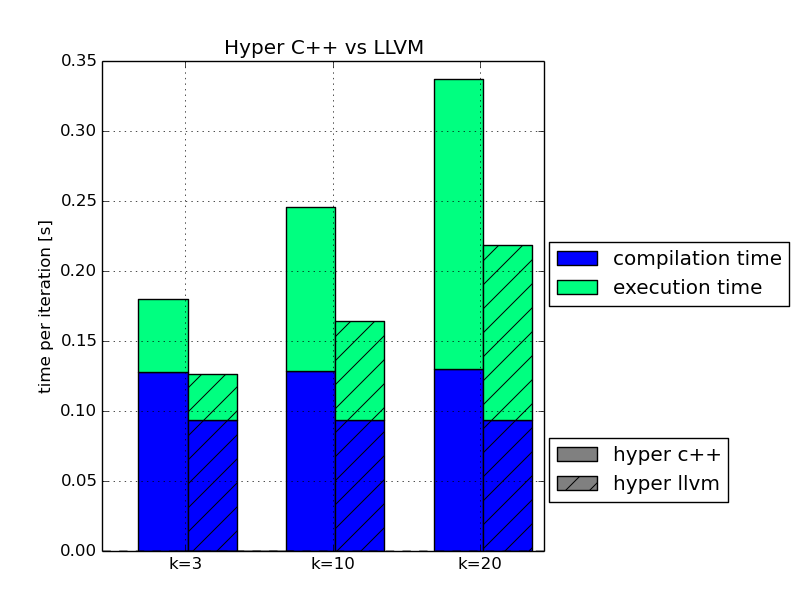
\includegraphics[scale=0.5, trim="0cm 1.5cm 0cm 0cm"]{figures/charts/hyper_50000}
  \caption[High Dimensional - Time per Iteration]{High Dimensional - Time per Iteration.}
  \label{fig:hyper_50000}
\end{figure}

Again, the compilation time stays constant for different values of $k$. The increase of compilation time compared to the previous network data set is induced by the high dimensionality: For each dimension additional code has to be generated. Therefore the code for a data set with four dimension is faster to compile than for a data set with 50 dimensions. 
The difference in the running time is similar to the network data set even though the increase in performance between the two implementations is not as significant. For $k = 3$, LLVM is faster by a factor 1.6 and for $k = 10$ and $k = 20$ by 1.7. This time the increase in execution time is strongly correlated. From $k = 3$ to $k = 10$, the LLVM version and the C++ version grow both by a factor of 2.2. From $k = 3$ to $k = 20$, the LLVM version grows by a factor of 4, while the C++ version grows by 3.8.
\\
Interestingly, the execution time for the network data set is lower than for the high dimensional data set, even though the network set has a size of 0.019 GB, while the high dimensional data set has only 0.009 GB. Even if we omit the compilation time which stays constant for a growing number of iterations and only look at the execution time the network data set is only for the C++ implementation and $k = 3$ slower than the high dimensional data set. Apparently, our implementation performs much better for low dimensional data sets, where not that much code has to be generated. As already mentioned, for each additional dimension additional code has to be generated and executed. For small data sets this compilation time can be a limiting factor, in addition to the extended execution time for high dimensional data sets in general.
\\
~\autoref{tab:med_serial} and~\autoref{tab:med_hd_serial} show the same experiment for the medium size and the medium size high dimensional data set. Both consist of 15 million instances, the first of four dimensions and the second of 50 dimensions. The compilation time of the medium size data set is similar to the network data set since both consist of four dimensions. The same is true for the medium size high dimensional data set and the previously used high dimensional data set: Both consist of 50 dimensions and the compilation time is quite similar. This shows us that the compilation time is independent of the data size and only affected by the number of dimensions. However, as the number of instances grows, the compilation time is not a significant factor for the overall running time anymore, as~\autoref{fig:hyper_15Mxhd} shows: The compilation time is not even visible plotting the data as stacked bar charts. 
\\
Again, the LLVM version shows a much better performance compared to the C++ version. For the medium size data set the overall running time is faster by a factor of 2.5, 1.6 and 1.4 for $k = 3, 10$ and 20, and for the medium size high dimensional data set by a factor of 1.6, 1.5 and 1.5, respectively.

\begin{table}[htsb]
  \caption[Medium Size - Time per Iteration]{Medium Size - Time per Iteration.}
  \label{tab:med_serial}
  \centering
  \begin{tabular}{l l l l l}
    \toprule
      & HyPer C++ & & HyPer LLVM & \\
      k & compilation[s] & execution[s] & compilation[s] & execution[s] \\
    \midrule
      3  & 0.0041 & 2.3779 & 0.0047 & 0.9191 \\
      10 & 0.0041 & 3.2856 & 0.0047 & 2.1001 \\
      20 & 0.0041 & 4.6765 & 0.0047 & 3.4518 \\
    \bottomrule
  \end{tabular}
\end{table}


\begin{table}[htsb]
  \caption[Medium Size High Dimensional - Time per Iteration]{Medium Size High Dimensional - Time per Iteration.}
  \label{tab:med_hd_serial}
  \centering
  \begin{tabular}{l l l l l}
    \toprule
      & HyPer C++ & & HyPer LLVM & \\
      k & compilation[s] & execution[s] & compilation[s] & execution[s] \\
    \midrule
      3  & 0.1127 & 16.2787 & 0.0935 & 10.3302 \\
      10 & 0.1127 & 34.0051 & 0.0935 & 22.0209 \\
      20 & 0.1126 & 59.2904 & 0.0935 & 38.7046 \\
    \bottomrule
  \end{tabular}
\end{table}

Obviously the execution time for the high dimensional data set is much larger compared to the low dimensional data set: This time the high dimensional data set has the same number of instances but 50 dimensions. For the C++ implementation the execution time is increased by a factor of 6.8 for $k = 3$, 10.3 for $k = 10$ and 12.6 for $k = 20$. For the LLVM implementation it is 11.2, 10.5, 11.2, respectively. Since the high dimensional data (2.79 GB) set is larger than the medium size data set (0.22 GB) by a factor of 12.7, the values are strongly correlated to the growth of the data set.

\begin{figure}[htsb]
  \centering
  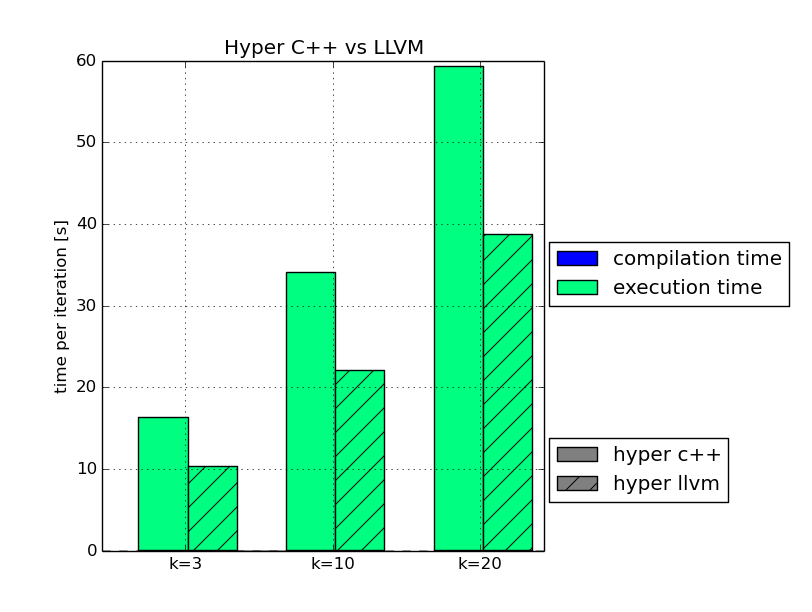
\includegraphics[scale=0.5, trim="0cm 1.5cm 0cm 0cm"]{figures/charts/hyper_15Mxhd}
  \caption[Medium Size High Dimensional - Time per Iteration]{Medium Size High Dimensional - Time per Iteration.}
  \label{fig:hyper_15Mxhd}
\end{figure}


Finally,~\autoref{tab:large_serial} shows the same experiment for the large size data set. The data set consists of ten dimensions and therefore the compilation time increases compared to the data sets with four dimensions by a factor of around two. However, since the data set has a size of 5.59 GB we can omit the compilation time since it does not affect the overall running time. Comparing the two versions regarding the overall running time, we observe that the LLVM version provides again much better results and is faster by a factor of 2.0, 1.5 and 1.4 for $k = 3, 10$ and 20 compared to the C++ implementation. This results in a difference of around 20 seconds per iteration between the two implementations.



\begin{table}[htsb]
  \caption[Large Size - Time per Iteration]{Large Size - Time per Iteration.}
  \label{tab:large_serial}
  \centering
  \begin{tabular}{l l l l l}
    \toprule
      & HyPer C++ & & HyPer LLVM & \\
      k & compilation[s] & execution[s] & compilation[s] & execution[s] \\
    \midrule
      3  & 0.0088 & 37.2804 & 0.0097 & 18.3734 \\
      10 & 0.0088 & 62.0034 & 0.0097 & 40.4783 \\
      20 & 0.0191 & 92.5868 & 0.0097 & 67.2364 \\
    \bottomrule
  \end{tabular}
\end{table}


In conclusion, we observed that the compilation time is not affected by the number of instances but the number of dimensions, where high dimensional data sets slow down the compilation phase. Interestingly, there is no significant difference regarding the compilation time between the two HyPer implementations. 
\\
Usually, the execution time outnumbers the compilation time by several factors. The only exception is the small, high dimensional data set as shown in the experiment. Here, the compilation time is slower than the execution time for small $k$. Furthermore the execution time grows by the number of instances and is much faster for the LLVM implementation. With equality regarding the compilation and a performance increase regarding the execution time the LLVM version was the best choice for all performed experiments and the implementation aspects should be used as building block for future HyPer operators for data mining.


\section{Performance Comparison with Competitor Systems}\label{section:performance}

In this section we compare our serial HyPer implementations with R and Julia’s implementation of the k-Means algorithm. As algorithm, the Lloyd algorithm with a maximum iteration number of ten is chosen. Apart from the large data set, the algorithm is executed 100 times for $k = 3, 10$ and $20$, respectively. For the large data set, the algorithm is executed ten times. The result is then presented as the execution time per iteration. For each algorithm the median, the 90th percentile and the 95th percentile are stated for each $k$. 

\begin{table}[htsb]
  \caption[3D Network - Time per Iteration]{3D Network - Time per Iteration in seconds.}
  \label{tab:network_all1}
  \centering
  \begin{tabular}{ll l l l |l l l |l l l |l l l}
    \toprule
      & & \multicolumn{3}{c}{Julia} & \multicolumn{3}{c}{R} & \multicolumn{3}{c}{HyPer C++} & \multicolumn{3}{c}{HyPer LLVM}  \\
      & \emph{k} & 3 & 10 & 20 & 3 & 10 & 20 & 3 & 10 & 20 & 3 & 10 & 20 \\
    \midrule
      \parbox[t]{2mm}{\multirow{3}{*}{\rotatebox[origin=c]{90}{\emph{percentile}}}} & 50  & 0.21 & 0.22 & 0.29 & 0.03 & 0.04 & 0.08 & 0.08 & 0.10 & 0.14 & 0.02 & 0.06 & 0.10 \\
      & 90  & 0.27 & 0.30 & 0.32 & 0.06 & 0.06 & 0.10 & 0.09 & 0.12 & 0.20 & 0.03 & 0.06 & 0.10 \\
      & 95  & 0.31 & 0.35 & 0.35 & 0.08 & 0.07 & 0.11 & 0.10 & 0.13 & 0.22 & 0.03 & 0.06 & 0.10 \\
    \bottomrule
  \end{tabular}
\end{table}

\begin{figure}[htsb]
  \centerline{
  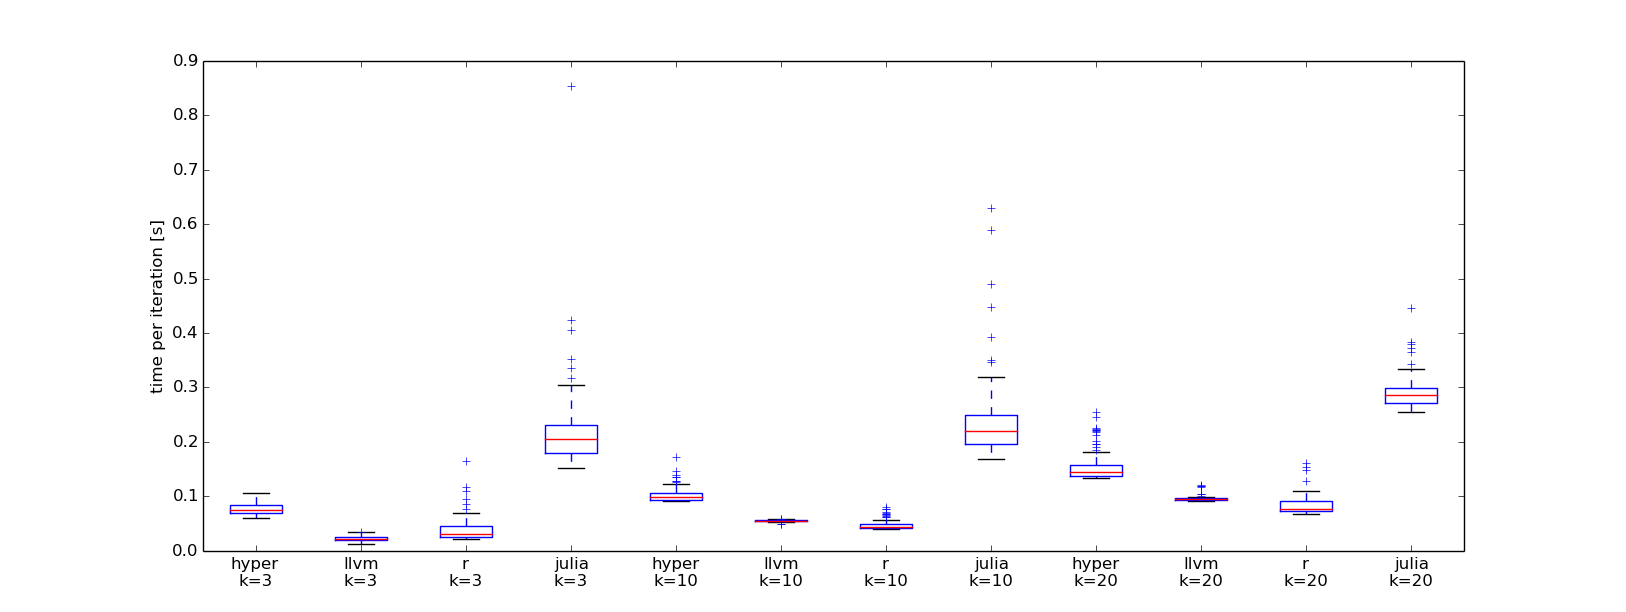
\includegraphics[scale=0.4, trim="0cm 1cm 0cm 0cm"]{figures/charts/network_all}
  }
  \caption[3D Network - Time per Iteration]{3D Network - Time per Iteration.}
  \label{fig:network_all}
\end{figure}

First, we test against the real world network data set. The result is presented in~\autoref{tab:network_all1}. As we already know, the HyPer LLVM implementation outnumbers the C++ version. For the median, the LLVM implementation is 3.4, 1.8 and 1.5 times faster for $k = 3, 10$ and $20$. Julia performs the slowest, our LLVM implementation is 9.5, 4.0 and 3.1 times faster, respectively. Only the R implementation can compete with the HyPer LLVM operator and is with 0.7, 0.8 and 0.8 for $k = 3, 10$ and 20 even a bit faster. However, all tested programs differ in a few hundred milliseconds therefore the differences are not very significant.
\\
~\autoref{fig:network_all} depicts the result as a boxplot. We observe that the C++ version, the LLVM version and R are closely together, while Julia lays behind. Also regarding the variance of the 100 runs, Julia shows the strongest variations and many outliers.

\begin{table}[htsb]
  \caption[High Dimensional - Time per Iteration]{High Dimensional - Time per Iteration in seconds.}
  \label{tab:highdim_all}
  \centering
  \begin{tabular}{l l l ll |l l l |l l l |l l l}
    \toprule
      && \multicolumn{3}{c}{Julia} & \multicolumn{3}{c}{R} & \multicolumn{3}{c}{HyPer C++} & \multicolumn{3}{c}{HyPer LLVM}  \\
      &\emph{k} & 3 & 10 & 20 & 3 & 10 & 20 & 3 & 10 & 20 & 3 & 10 & 20 \\
    \midrule
      \parbox[t]{2mm}{\multirow{3}{*}{\rotatebox[origin=c]{90}{\emph{percentile}}}} &50  & 0.04 & 0.05 & 0.07 & 0.03 & 0.05 & 0.08 & 0.18 & 0.24 & 0.35 & 0.13 & 0.16 & 0.22 \\
      &90  & 0.04 & 0.05 & 0.07 & 0.04 & 0.06 & 0.10 & 0.21 & 0.34 & 0.40 & 0.13 & 0.16 & 0.22 \\
      &95  & 0.04 & 0.05 & 0.07 & 0.05 & 0.07 & 0.11 & 0.22 & 0.35 & 0.44 & 0.13 & 0.17 & 0.22 \\
    \bottomrule
  \end{tabular}
\end{table}

\begin{figure}[htsb]
  \centerline{
  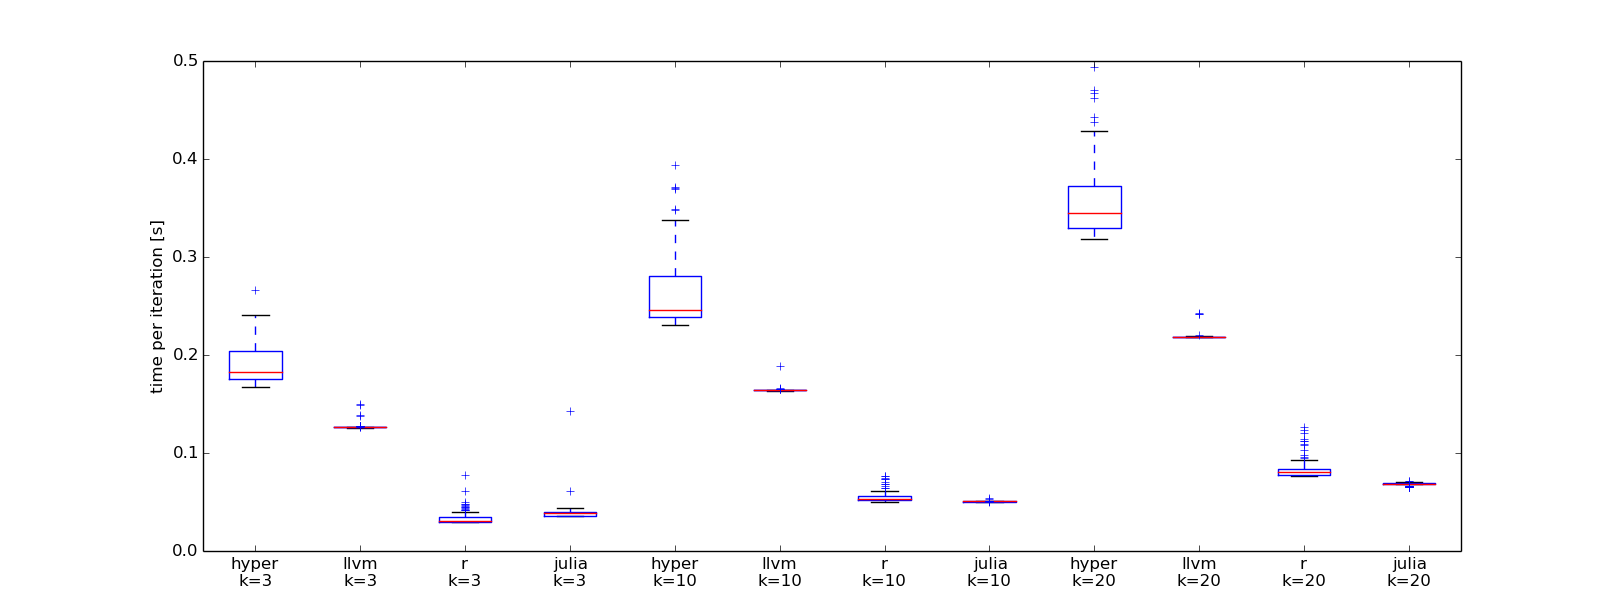
\includegraphics[scale=0.4, trim="0cm 1cm 0cm 0cm"]{figures/charts/50000_all}
  }
  \caption[High Dimensional - Time per Iteration]{High Dimensional - Time per Iteration.}
  \label{fig:50000_all}
\end{figure}



Performing the same experiment on the high dimensional data set we see a different result, as depicted in~\autoref{tab:highdim_all}. As already shown, the HyPer C++ and LLVM versions are slower compared to the network data set even though the data set is smaller by size. R takes almost the same time for both data sets. Interestingly, Julia’s k-Means algorithm is now as fast as the R implementation, for $k = 10$ and 20 it is even faster. This is also depicted by the boxplot in~\autoref{fig:50000_all}. Also the variance changed: The HyPer C++ version shows the highest variance with many outliers, while Julia's variance is very small this time.   
\\
This result gives us interesting knowledge about the different implementations. Both HyPer operators perform poorly when dimensions increase. An increase in dimensions and a decrease in instances does not affect R significantly. On the other hand, Julia shows much better results as dimensions increase and seems to be optimized for high dimensions: It is 5.4, 4.4 and 4.2 times faster for $k = 3, 10$ and 20 on the high dimensional set compared to the network data set, and the variance is much lower. A conversation with Prof. Timothy E. Holy, Ph.D. substantiated this hypothesis\footnote{Julia User Group:~\url{http://bit.ly/1anXGMF}, 25.01.2015.}. 

\begin{table}[htsb]
  \caption[Medium Size - Time per Iteration]{Medium Size - Time per Iteration in seconds.}
  \label{tab:medium_all}
  \centering
  \begin{tabular}{l l l ll |l l l |l l l |l l l}
    \toprule
      && \multicolumn{3}{c}{Julia} & \multicolumn{3}{c}{R} & \multicolumn{3}{c}{HyPer C++} & \multicolumn{3}{c}{HyPer LLVM}  \\
      &\emph{k} & 3 & 10 & 20 & 3 & 10 & 20 & 3 & 10 & 20 & 3 & 10 & 20 \\
    \midrule
      \parbox[t]{2mm}{\multirow{3}{*}{\rotatebox[origin=c]{90}{\emph{percentile}}}} &50  & 5.42 & 7.61 & 10.62 & 0.77 & 1.61 & 2.50 & 2.38 & 3.29 & 4.68 & 0.92 & 2.10 & 3.46 \\
      &90  & 5.43 & 7.65 & 10.71 & 0.79 & 1.63 & 2.55 & 2.57 & 3.44 & 4.77 & 0.94 & 2.14 & 3.51 \\
      &95  & 5.44 & 7.70 & 10.91 & 0.80 & 1.63 & 2.56 & 2.64 & 3.45 & 4.84 & 0.94 & 2.14 & 3.52 \\
    \bottomrule
  \end{tabular}
\end{table}

\begin{table}[htsb]
  \caption[Medium Size HD - Time per Iteration]{Medium Size HD - Time per Iteration in seconds.}
  \label{tab:medium_hd_all}
  \centering
  \begin{tabular}{lllll|l l l|l l l|l l l}
    \toprule
      & & \multicolumn{3}{c}{Julia} & \multicolumn{3}{c}{R} & \multicolumn{3}{c}{HyPer C++} & \multicolumn{3}{c}{HyPer LLVM}  \\
      & \emph{k} & 3 & 10 & 20 & 3 & 10 & 20 & 3 & 10 & 20 & 3 & 10 & 20 \\
    \midrule
      \parbox[t]{2mm}{\multirow{3}{*}{\rotatebox[origin=c]{90}{\emph{percentile}}}} & 50  & 11.46 & 15.69 & 21.67 & 9.43 & 15.48 & 23.77 & 16.39 & 34.12 & 59.40 & 10.42 & 22.11 & 38.80 \\
     & 90  & 11.51 & 15.81 & 21.69 & 9.50 & 15.50 & 23.79 & 16.77 & 36.11 & 59.53 & 10.44 & 22.12 & 38.84 \\
     & 95  & 11.65 & 15.83 & 21.70 & 9.64 & 15.58 & 23.79 & 17.29 & 42.15 & 59.57 & 10.45 & 22.13 & 38.84 \\
    \bottomrule
  \end{tabular}
\end{table}


\begin{figure}[htsb]
  \centerline{
    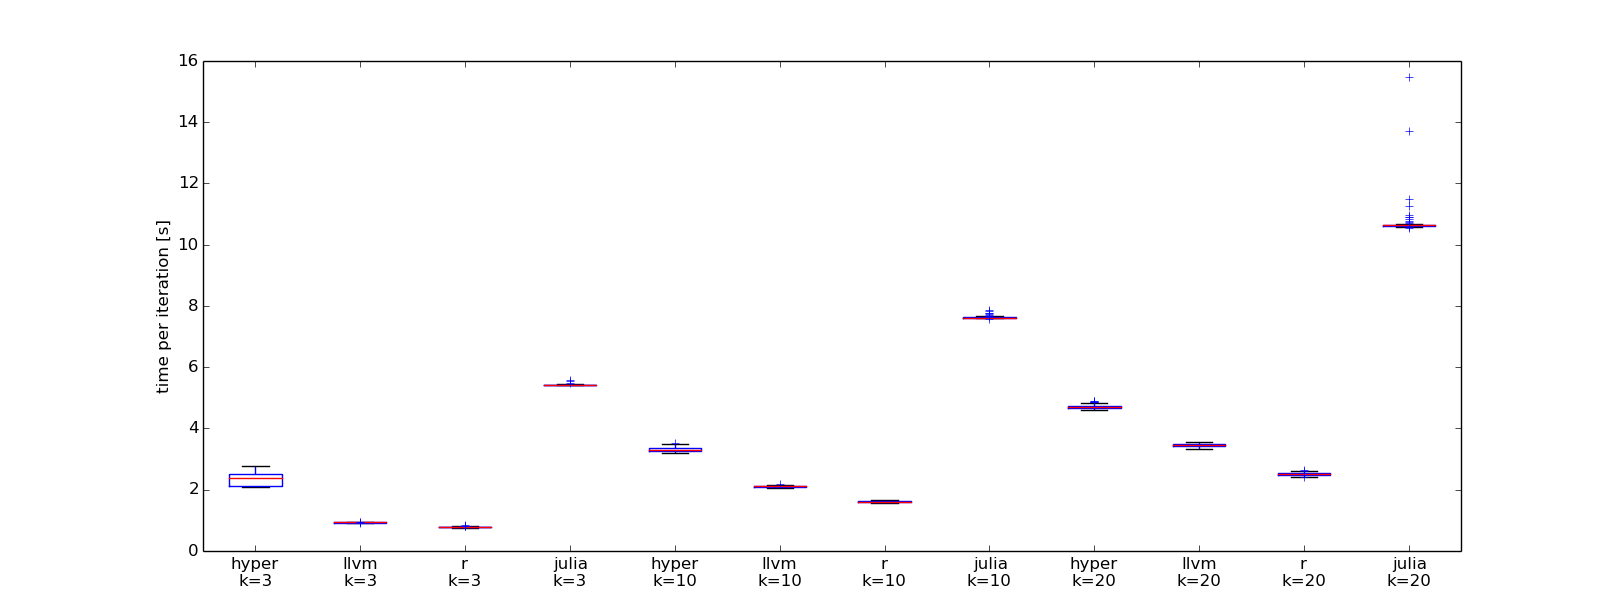
\includegraphics[scale=0.4, trim="0cm 1cm 0cm 0cm"]{figures/charts/15M_all}
  }
  \caption[Medium Size - Time per Iteration]{Medium Size - Time per Iteration.}
  \label{fig:15M_all}
\end{figure}


\begin{figure}[htsb]
  \centerline{
    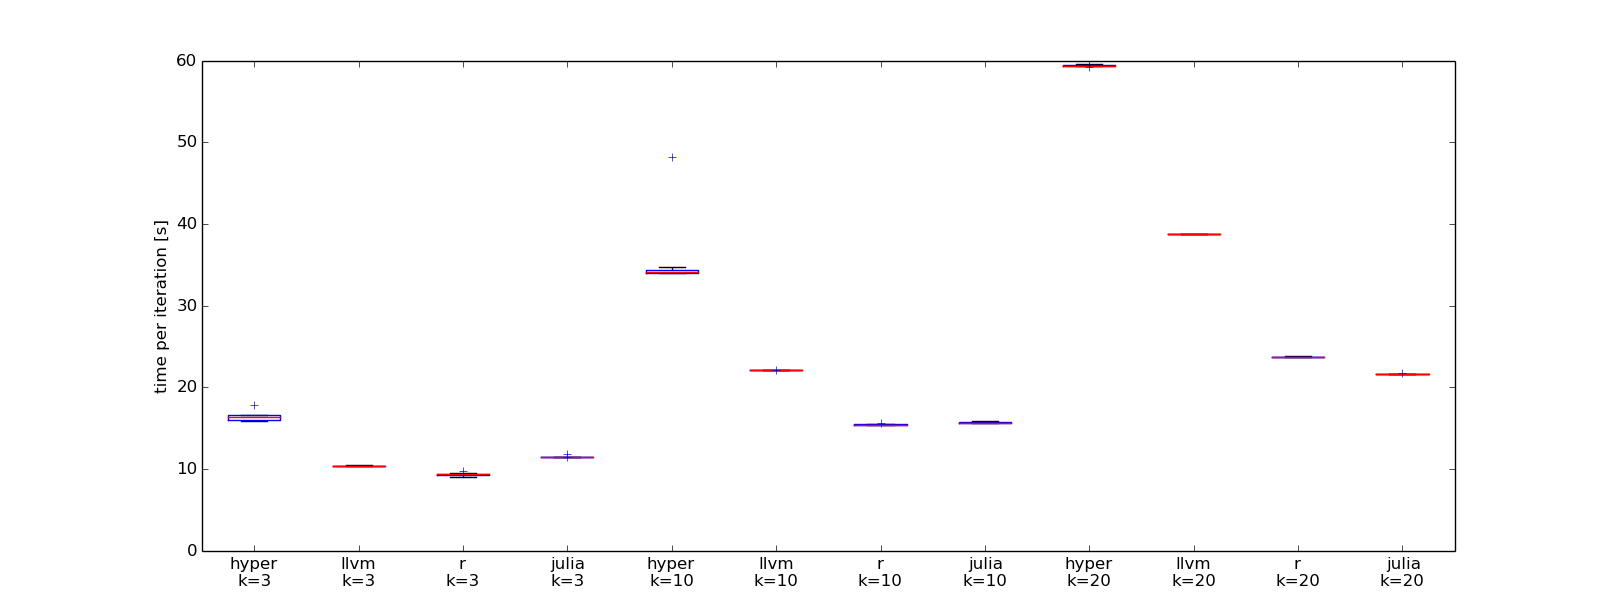
\includegraphics[scale=0.4, trim="0cm 1cm 0cm 0cm"]{figures/charts/15Mxhd_all}
  }
  \caption[Medium Size HD - Time per Iteration]{Medium Size HD - Time per Iteration.}
  \label{fig:15Mxhd_all}
\end{figure}



We perform the same experiment on the medium size and the medium size high dimensional data set.~\autoref{tab:medium_all} shows the result of the medium size data set. Again, the LLVM version is faster than the C++ version by a factor of 2.5, 1.6 and 1.4 for $k = 3, 10$ and $20$. Since the dataset has only four dimensions Julia performs poorly and is by a factor of 5.9, 3.6 and 3.1 slower compared to the LLVM version. As for the network data set R demonstrates the best performance and is faster than LLVM by a factor of 0.8, 0.8 and 0.7 for $k = 3, 10$ and 20. Again we depict the result as a boxplot in~\autoref{fig:15M_all}, where we observe a small variance for all used tools; only Julia has a few outliers for $k = 20$.
\\
In comparison,~\autoref{tab:medium_hd_all} and ~\autoref{fig:15Mxhd_all} depict the result for the medium size high dimensional data set. As before, the HyPer implementation does not perform ideally on high dimensions. For $k = 3$, the LLVM version is slower than R by a factor of 0.9 but faster than Julia by a factor of 1.1. However, as $k$ grows, R and Julia show slightly better results. Both show a speed up by a factor of 0.7 for $k = 10$, and 0.6 for $k = 20$, compared to the LLVM version. 
\\
Obviously the high dimensional data set takes more time per iteration having the same number of instances with a lot more dimensions. However, Julia shows a slow down by a factor of only 2 for all $k$'s, although the dimensions increase from 4 to 50; R shows a slow down by a factor of 12 for $k = 3$, and 10 for $k = 10$ and 20, the C++ version by a factor of 7, 10, 13 for $k = 3, 10$ and 20, and the LLVM version by a factor of 11 for all $k$'s. Julia performs again the best for high dimensional data. R and HyPer's LLVM operator behave very similar this time. An explanation is that the compilation time is not a limiting factor anymore for the LLVM implementation: For the high dimensional data set with 50,000 instances the compilation time was higher than the execution time. This time the data set consists of 15 million tuples therefore the poor compilation time does not affect the overall performance anymore.
\\
As final test we perform the same experiment on the large data set containing 150 million instances, as shown in~\autoref{tab:150M_all}. This time the HyPer LLVM implementation outnumbers all the other tools, the C++ version by a factor of 2.0, 1.5 and 1.4 for $k = 3, 10$ and 20, Julia by a factor of 3.6, 2.2, 2.0, respectively, and even R by a factor of 1.6, 1.2 and 1.1, respectively. For growing $k$, the R implementation comes very close to the HyPer LLVM version. This result is also depicted in the boxplot in~\autoref{fig:150M_all}.
\\
In conclusion, the experiments demonstrate that the HyPer k-Means operator can compete with state-of-the-art tools for clustering. Particularly the LLVM implementation demonstrates good performance and shows similar results as the R implementation of the k-Means algorithm. However, for high dimensional data sets both HyPer operators do not perform ideally and are outnumbered by Julia's implementation optimized for high dimensions. Here is potential for future optimization as we demonstrate in Section~\ref{section:parallel} with a parallel implementation. Yet, if we take into account that the k-Means algorithm runs on top of an entire database with all its overhead, these results are supporting further development and the implementation of other data mining algorithms as HyPer operators. 




\begin{table}[htsb]
  \caption[Large Size - Time per Iteration]{Large Size - Time per Iteration in seconds.}
  \label{tab:150M_all}
  \centering
  \begin{tabular}{l l l ll |l l l |l l l |l l l}
    \toprule
      && \multicolumn{3}{c}{Julia} & \multicolumn{3}{c}{R} & \multicolumn{3}{c}{HyPer C++} & \multicolumn{3}{c}{HyPer LLVM}  \\
      &\emph{k} & 3 & 10 & 20 & 3 & 10 & 20 & 3 & 10 & 20 & 3 & 10 & 20 \\
    \midrule
      \parbox[t]{2mm}{\multirow{3}{*}{\rotatebox[origin=c]{90}{\emph{percentile}}}} &50  & 65.62 & 90.37 & 132.39 & 29.47 & 48.21 & 72.40 & 37.29 & 62.01 & 92.60 & 18.38 & 40.49 & 67.25 \\
      &90  & 65.72 & 92.01 & 135.87 & 30.80 & 54.73 & 77.27 & 37.50 & 62.41 & 92.86 & 18.44 & 40.72 & 67.57 \\
      &95  & 65.78 & 92.27 & 137.21 & 33.08 & 55.02 & 77.97 & 37.52 & 62.72 & 92.95 & 18.46 & 40.72 & 67.63 \\
    \bottomrule
  \end{tabular}
\end{table}





\begin{figure}[htsb]
  \centerline{
    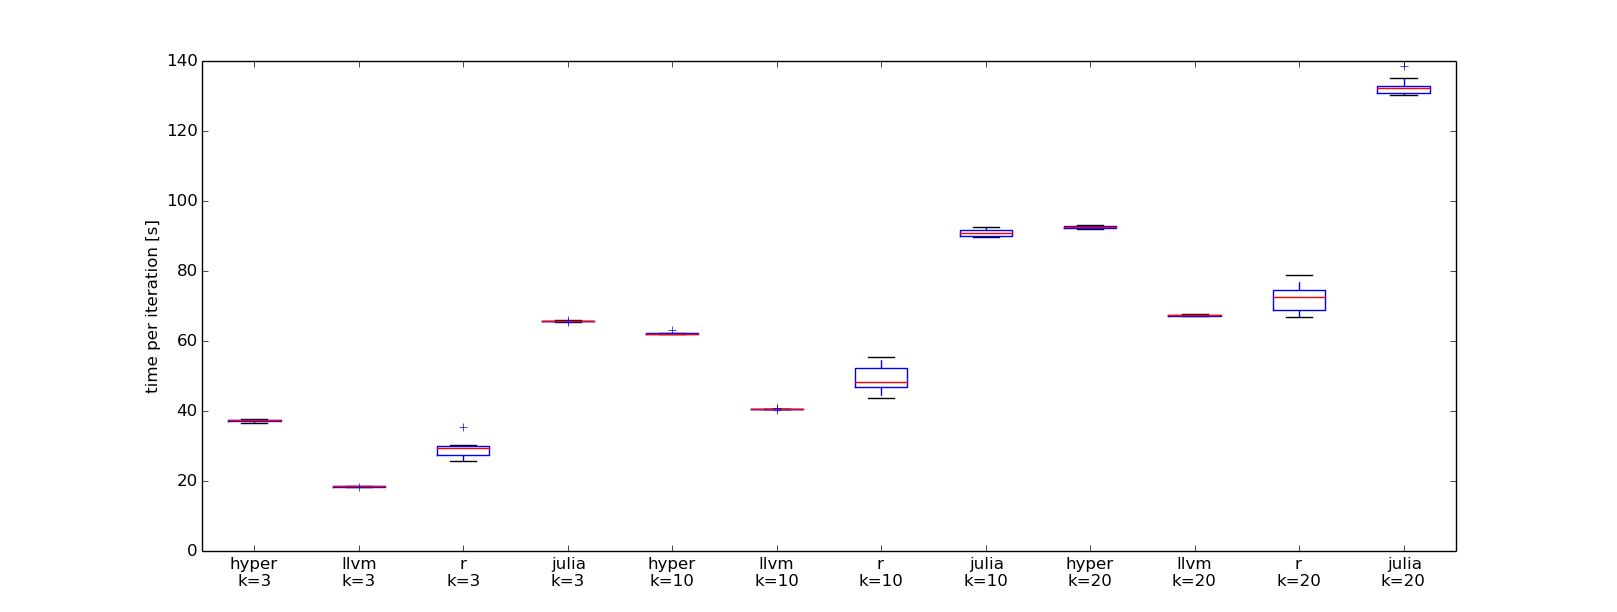
\includegraphics[scale=0.4, trim="0cm 1cm 0cm 0cm"]{figures/charts/150M_all}
  }
  \caption[Large Size - Time per Iteration]{Large Size - Time per Iteration.}
  \label{fig:150M_all}
\end{figure}



\section{Parallel Implementation}\label{section:parallel}


So far we have only covered the serial implementations of the HyPer k-Means operator: In Section~\ref{section:serial}  we figured out that the LLVM implementation outperforms the C++ version on all used data sets. In Section~\ref{section:performance} we compared the performance against Julia and R and showed that HyPer is able to compete with state-of-the-art technologies for data mining.
\\
However, as data sets grow serial execution takes more and more time, making real-time data mining almost impossible. Furthermore, we do not exploit the possibilities of modern database hardware and the advantages of multi-threaded execution of algorithms. To address these challenges we presented a parallel implementation of the HyPer k-Means operator in Section~\ref{section:parallel_implementation}. In this section we compare this parallel implementation with the LLVM version and the R implementation. Both tools demonstrate the best results on the medium size, the medium size high dimensional and the large data set. Julia and the C++ driven implementation are excluded in this section since their performance is either similar or slower to R and the LLVM implementation on the used data sets.

\begin{table}[htsb]
  \caption[Medium Size - Time per Iteration]{Medium Size - Time per Iteration in seconds.}
  \label{tab:medium_final}
  \centering
  \begin{tabular}{l l l ll |l l l |l l l }
    \toprule
      && \multicolumn{3}{c}{R} & \multicolumn{3}{c}{HyPer LLVM} & \multicolumn{3}{c}{HyPer Parallel}  \\
      &\emph{k} & 3 & 10 & 20 & 3 & 10 & 20 & 3 & 10 & 20 \\
    \midrule
      \parbox[t]{2mm}{\multirow{3}{*}{\rotatebox[origin=c]{90}{\emph{percentile}}}} &50  & 0.77 & 1.61 & 2.50 & 0.92 & 2.10 & 3.46 & 1.35 & 1.52 & 1.75 \\
      &90  & 0.79 & 1.63 & 2.55 & 0.94 & 2.14 & 3.51 & 1.38 & 1.53 & 1.84 \\
      &95  & 0.80 & 1.63 & 2.56 & 0.94 & 2.14 & 3.52 & 1.40 & 1.53 & 1.85 \\
    \bottomrule
  \end{tabular}
\end{table}

~\autoref{tab:medium_final} shows the result as the time per iteration for $k = 3, 10$ and 20. As before, the median, the 90th and 95th percentile are presented. For $k = 3$, we surprisingly observe that both the R and the LLVM version are faster than the parallel version. However, as $k$ grows, the parallel version outperforms R and the LLVM version. This circumstance is also shown in the bar chart in~\autoref{fig:final_15M}.
\\
The reason is that for the parallel execution the running time is almost independent of $k$ because the computation is performed on different, independent threads that are only slightly affected by an increase of $k$. However, if $k$ would even further grow while the number of cores stays constant, the performance might be affected also in the parallel execution mode. For a $k$ between 3 and 20 this does not happen and therefore the parallel version outperforms R and LLVM. For R, the time per iteration grows by a factor of 2.1 from $k = 3$ to $k = 10$, and by a factor of 1.6 from $k = 10$ to $k = 20$. For LLVM we observe an increase by a factor of 2.3 and 1.6, respectively. In contrast, the parallel implementation grows only by factor of 1.1 and 1.2, respectively. In other words, R and the LLVM version grow by seconds as $k$ grows, while the parallel version grows insignificantly by around 200 milliseconds. 

\begin{figure}[htsb]
  \centering
  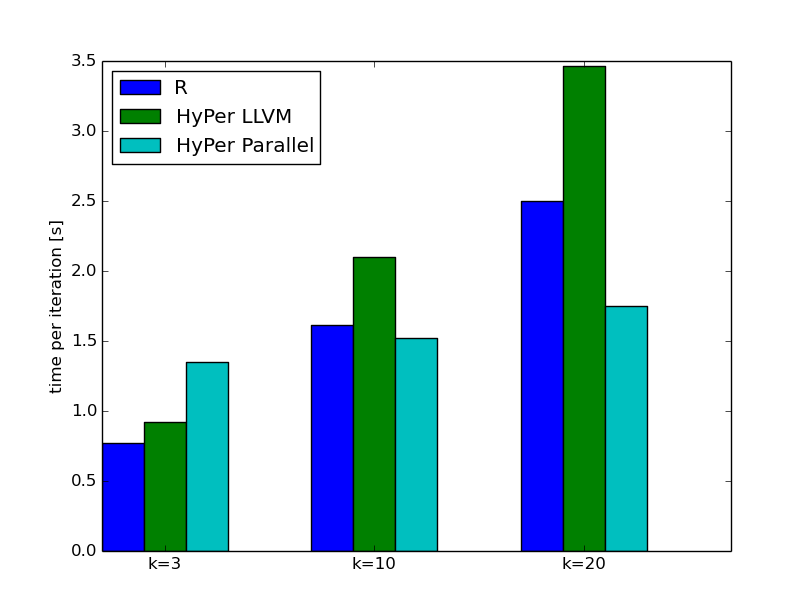
\includegraphics[scale=0.5, trim="0cm 1.5cm 0cm 0cm"]{figures/charts/final_15M}
  \caption[Medium Size - Time per Iteration]{Medium Size - Time per Iteration in seconds.}
  \label{fig:final_15M}
\end{figure}

~\autoref{tab:medium_hd_final} shows the same experiment on the medium high dimensional data set. For this data set the parallel version outperforms the other two implementations for all $k$'s, even for $k = 3$.~\autoref{fig:final_15_hd} depicts that the parallel version is again almost independent of $k$, in contrast to R and LLVM. R grows by a factor of 1.6 from $k = 3$ to $k = 10$, and 1.5 from $k = 10$ to $k = 20$; for LLVM we observe an increase by a factor of 2.1 and 1.8, respectively, and for the parallel version a factor of 1.4 and 1.4, respectively. 
\\
Even though the parallel version is not as independent of the cluster number $k$ as for the low dimensional data set, the increase in time is much lower. Additionally, a performance gain is achieved by the ability to handle high dimensional data better: From four dimensions to 50 dimensions, the parallel execution time is only affected by a factor of 4.3, 5.3 and 6.5 for $k = 3, 10$ and 20. R and LLVM are affected by a much larger factor: 12.3, 9.6 and 9.5 for R, and 11.3, 10.5 and 11.2 for the LLVM implementation. Again, the performance benefits from the parallel execution: Computing the distance from each data point to each center point is computationally expensive, even more when the instances consist of many dimensions. Then, a computation on many, independent threads speeds up the performance tremendously, as shown in this experiment. 


\begin{table}[htsb]
  \caption[Medium Size HD - Time per Iteration]{Medium Size HD - Time per Iteration in seconds.}
  \label{tab:medium_hd_final}
  \centering
  \begin{tabular}{l l l ll |l l l |l l l }
    \toprule
      && \multicolumn{3}{c}{R} & \multicolumn{3}{c}{HyPer LLVM} & \multicolumn{3}{c}{HyPer Parallel}  \\
      &k & 3 & 10 & 20 & 3 & 10 & 20 & 3 & 10 & 20 \\
    \midrule
      \parbox[t]{2mm}{\multirow{3}{*}{\rotatebox[origin=c]{90}{\emph{percentile}}}} &50  & 9.43 & 15.48 & 23.77 & 10.42 & 22.11 & 38.80 & 5.84 & 8.04 & 11.30 \\
      &90  & 9.50 & 15.50 & 23.79 & 10.44 & 22.12 & 38.84 & 5.88 & 8.26 & 11.35 \\
      &95  & 9.64 & 15.58 & 23.79 & 10.45 & 22.13 & 38.84 & 5.88 & 8.29 & 11.37 \\
    \bottomrule
  \end{tabular}
\end{table}



\begin{figure}[htsb]
  \centering
  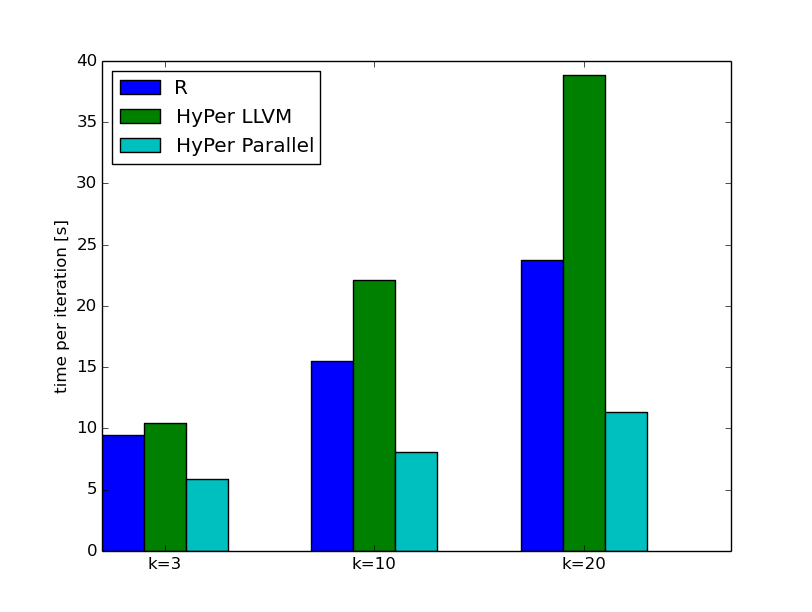
\includegraphics[scale=0.5, trim="0cm 1.5cm 0cm 0cm"]{figures/charts/15Mxhd_final}
  \caption[Medium Size HD - Time per Iteration]{Medium Size HD - Time per Iteration.}
  \label{fig:final_15_hd}
\end{figure}

Finally,~\autoref{tab:large_final} shows the result of the same experiment on the large size data set. Again, the parallel version is the fastest. For $k = 3$, the parallel version is faster than R by a factor of 1.8 and for LLVM by a factor of 1.1. For $k = 10$ the factors are even larger, 2.4 for R and 2.0 for LLVM, and 3.0 and 2.8 for $k = 20$, respectively. Again $k$ affects the performance of the parallel version only slightly, therefore the speed up is increasing as $k$ increases.
\\
To conclude, the parallel version performs much better than the LLVM and R implementation. Except for the medium size data set and $k = 3$ it demonstrates always better results. However, since we are using only 16 cores even a higher speed up would be possible, in particular for larger data sets, more dimensions and a growing $k$. Furthermore, we are using the serial C++ version of the HyPer k-Means operator as foundation for our parallel implementation. As seen in the previous sections, this implementation performs poorly compared to the LLVM implementation: As in the serial implementation there are many function calls between the \texttt{runtime} and the \texttt{compile time system} also in the parallel version. Additionally, we are using high-level C++ constructs over the more efficient LLVM code generation. Therefore, in future implementations the LLVM version should be the building block of the parallel version which might lead to crucial performance improvements as observed already between the two serial implementations. And finally, only the computation of the distances is parallelized so far, while the recalculation of the cluster centers is still performed in serial. Therefore, we can expect even better results when we enhance the addressed shortcomings in future versions.


\begin{table}[htsb]
  \caption[Large Size - Time per Iteration]{Large Size - Time per Iteration in seconds.}
  \label{tab:large_final}
  \centering
  \begin{tabular}{l l l l l |l l l |l l l }
    \toprule
      && \multicolumn{3}{c}{R} & \multicolumn{3}{c}{HyPer LLVM} & \multicolumn{3}{c}{HyPer Parallel}  \\
      \emph{k} & 3 & 10 & 20 & 3 & 10 & 20 & 3 & 10 & 20 \\
    \midrule
      \parbox[t]{2mm}{\multirow{3}{*}{\rotatebox[origin=c]{90}{\emph{percentile}}}} &50  & 29.47 & 48.21 & 72.40 & 18.38 & 40.49 & 67.25 & 16.71 & 19.79 & 24.03 \\
      &90  & 30.80 & 54.73 & 77.27 & 18.44 & 40.72 & 67.57 & 16.94 & 20.13 & 24.33 \\
      &95  & 33.08 & 55.02 & 77.97 & 18.46 & 40.72 & 67.63 & 17.01 & 20.17 & 24.36 \\
    \bottomrule
  \end{tabular}
\end{table}




\begin{figure}[htsb]
  \centering
  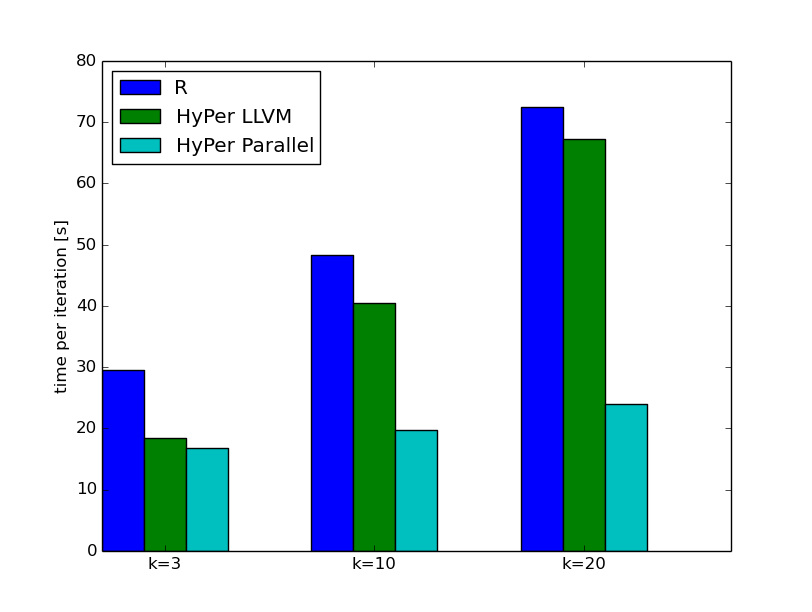
\includegraphics[scale=0.5, trim="0cm 1.5cm 0cm 0cm"]{figures/charts/final_150M}
  \caption[Large Size - Time per Iteration]{Large Size - Time per Iteration.}
  \label{fig:final_150M}
\end{figure}

\chapter{Conclusions and Future Work}\label{chapter:conclusion}


\section{Conclusions}

\section{Future Work}

Many open challenges remain in mining data in HyPer. In this section we discuss this future work and begin with general improvements for the k-Means algorithm.
\\
Our k-Means implementation can take up to three input parameters: The cluster number k, the maximum number of iterations and a verbose option to output statistics about the algorithm execution. For the future we want to enhance the behaviour of k-Means and make our algorithm more flexible. That can be done by allowing the user to choose a distance function. For now, k-Means implements a Euclidean distance, however, for some problems other distances are more appropriate. Therefore we should offer to use the Manhattan, Euclidean, Minkowski and Chebyshev distance as well as the cosine similarity.
\\
Applying normalization before data clustering can improve the final result. This can be either implemented as input parameter for the k-Means algorithm or even better as standalone operator since other data mining algorithms can benefit from a normalization too.
\\
For big data sets the execution time of the k-Means algorithms can be quite high. The reasons is that the iterations has to take many iterations until it converges. An enhancement is an earlier termination: Usually, k-Means terminates if the clusters do not change anymore. However, for large data sets this could be a problem if a few data points are moving from cluster to cluster while the majority of data points remains constant. Nevertheless, an additional iteration of the algorithms has to be initiated. Therefore an additional input parameter can specify a tolerable change of data points. Is the change of data points underneath this border, the algorithm terminates even though there is a slight chance to find a better clustering.
\\
Heterogenous data is another problem for our algorithms. No all data sets consist only of numeric data. Often it is a mixture between numeric, binary and categorical attributes. An improvement is to first convert the binary and categorical to numeric attributes, and then improve the distance and cost function to keep the different dimensions comparable, as proposed in k-Means Mixed.
\\
Instead of implementing a new cost function the existing distance function can be improved by assigning a weight to each dimension. This is not only useful for mixed data sets but also for numerical attributes only. Assigning weights is not only possible for dimensions - also instance can be weighted differently since some are more significant than others.
\\
K-Means is usually implemented as the Lloyd algorithm, resulting in reasonable results. However, the execution time can be improved implementing the Hartigan-Wong algorithm. In contrary to the Lloyd algorithm it updates the centroids at any time a point is moved and makes time-saving choices for finding the closest cluster.
\\

So far, the result of k-Means is a table with an additional column specifying the cluster number. Since this table is returned using the consume function, it can be used on further SQL statements. The statistical information however, such as the final center coordinates or the number of iterations is only printed to the console. Therefore this information is lost and cannot be used in further SQL statements. A way forward is to generate additional tables storing the statistical information of a clustering. In this tables more information can be stored in an accessible way, e.g. the final center coordinates, the distance from each data point to its closest center and all statistical information. Up to now HyPer is only able to push tuples to the next consume operator and cannot generate additional tables. Since this information is very valid to analyze the k-Means result an extension of the existing operator model is suggested. Almost all data mining algorithms produce several additional intermediate and final results, thus this is a big step for computational data mining on databases.
\\
HyPer is a database system that makes already extensive use of index structures. Therefore an option is to improve the k-Means algorithms, e.g. by using nearest neighbour data structures when clustering high dimensional data.
\\
As shown in the evaluation chapter the LLVM implementation is much faster than the C++ version. Therefore, the center initialization using the k-Means++ method could benefit from a pure LLVM implementation instead of a C++ implementation with slow getDistance call for the center selection process.
\\
We have also shown the advantages of parallel execution of the k-Means algorithms. However, for small k and medium size data sets the parallel execution is still slower than the LLVM implementation. One reason is that the C++ version was used as parallel version leading to many calls from the runtime to the compile time system. A parallel implementation in LLVM code could tremendously boost the performance of the algorithm. Also the parallelization itself can be improved: Only the process of computing the distances is parallelized so far. While this is already a big performance improvement the algorithm would even benefit more from a parallel execution of the initialization process and of the updating of the cluster centers.
\\
For finding a ready market in the data scientist community it will be necessary to provide a functional language for executing the k-Means algorithm since not all data scientist might be fluent in SQL scripting languages. However, this is a challenge that goes beyond the implementation of a k-Means algorithm as a language has to be found that adapts all the available SQL expressions and operators of HyPer.
\\
The next point goes in the same direction: Data scientists do not only want to use the output as a database table or in a data structure of the functional language but also in a visual way. Therefore the HyPer system and its functional language must be able to connect with a 2D plotting library to produce publication quality figures in a variety of forms. For the k-Means clustering algorithms this means a possibility to plot the data points, e.g. as a scatter plot. An example for a 2D plotting library based on a functional language is the Python library matplotlib. 
\\
To fulfil the aim to provide further algorithms for data mining, it is appropriate to use the existing k-Means algorithm as building block. A very similar partitional clustering algorithm is the k-Medoids algorithm. In contrary to k-Means it chooses data points as centers instead of the mean of the mass of all assigned data points. This makes the algorithm more robust for handling outliers. As implementation, the existing k-Means algorithm can be reused, only the way of computing center points after data point assignment has to change according to the requirements of k-Medoids. 
\\
So far we assign each object to one distinct cluster. However, objects may belong to several clusters. The Expectation–maximization (EM) algorithm is very similar to the k-Means algorithm and has a focus on fuzzy clustering. As a long term goal, we want to include also algorithm for mining frequent patterns and association rules, classification and outlier detection. 
information.











% TODO: add more chapters here

\appendix{}

 % TODO: remove if glossary not needed
\glsaddall{} % add all defined terms to glossary, even if not referenced in text
\printglossaries{}

\microtypesetup{protrusion=false}
\listoffigures{}
\listoftables{}
\microtypesetup{protrusion=true}
\printbibliography{}

\end{document}
